\renewcommand\labelenumi{(\roman{enumi})}
\renewcommand\theenumi\labelenumi

\chapter{Local market services and products for active network management}
\label{chapterMarkets}

\chaptermark{Local Markets}
\section{Introduction}
There are many concepts in the field of power markets that are being formulated at the current time: local electricity markets, local markets, local power markets, smart city marketplaces, micro markets, microgrid energy markets, etc.. There is a need to set up the basis of these concepts, to build up the technology that enhances the transition towards a smart grid based on the distribution of locally generated energy instead of big power plants.
This chapter aims to provide the reader with a standardized theoretical background of local and micro power markets so he or she can understand all the agents involved in the energy transition, and thus further research in this field might be performed. Several references are included to prove that right now this topic is of broad and current interest, with many ongoing projects involved.
To start with, the reader will start by asking himself or herself whether there is a need to develop local and micro power markets.
In this chapter, the concepts of local and micro power markets are reviewed and then defined to establish a common reference for their development. The literature review aims to provide an overview of the current status of local and micro power markets. The differences between local and micro power markets are highlighted, based on the literature reviews regarding market design, services, and approach.

\begin{figure}[]
	\centering
	\includegraphics[width=0.7\columnwidth ]{ChapterMarkets/Figures/intro_figure_i.pdf}
	   %\vspace*{-8cm}
		\caption{Chapter objective based on the PhD scope}
	\label{fig:chapter_obj}  
\end{figure}

\section{Why Local and Micro?} \label{sec:why}
The road to local and micro markets comes after years of a centralized market and a rigid structure of the electric power system. Despite this, at present society is facing a globalization movement, where the objective is to simplify entities and structures, and achieve a more homogeneous behaviour of the markets, developing a model that is more predictable, more standardized, and more transparent \cite{Mallet2014}. Besides the energy transition,there is a challenge for distribution system operators (DSO): to connect more than 90% of customers and ever-growing numbers of DERs in a rapidly changing, ever more decentralized, and digital energy world. One
example of this behaviour is the project EUPHEMIA \cite{EUPHEMIA2016}, where the aim is to develop a single price-coupling algorithm, used to calculate energy allocation and electricity prices across Europe, maximizing the overall welfare and increasing the transparency of the prices and flows computations. So why is there a need to go local and micro in terms of energy markets? What advantages does this approach have? The objective of this chapter is to answer the questions faced in \cite{DesignElectricityMarketRossetoo2017}:

\begin{tcolorbox}
To what extent do these concepts offer something new? Aren't these services already offered by suppliers, who can exchange flexibility and energy with consumers, and help them in home automation? Don't current regulation, market arrangements and commercial
practices already allow all this? How can the proposed solutions be made compatible with the natural monopoly of the grid, and deal with the likely conflicts of interest? In activities that present significant economies of scale, thanks to the power of digital devices, what is the advantage of being local and small scale?
\end{tcolorbox}

One of the advantages of being local and small scale is to fulfil the preferences of consumers, as is stated in \cite{faber2014micro}. For instance, some consumers are willing to pay more for the energy they consume if the energy they receive meets their environmental preferences, such being carbon-free, pollution-free, exclusively renewable and locally generated \cite{lane2013costing}. The fact is that the structure and roles of transmission and distribution systems are changing significantly due to the integration of renewable energy sources (RES), in a distributed way, in both transmission and distribution grids. The integration of these DERs along the distribution grid creates local variations that can affect the optimal operation of transmission and distribution networks.

Despite this, local supply variation can be matched with local demand variation, resulting in a local way to solve the problem \cite{mengelkamp2018designing} and producing a potential business model to increase the hosting capacity of the distribution grid without investing in it. This could be the basic idea of a local or micro power market. At present, the existing electricity markets (e.g. wholesale market, balancing market, futures market, and bilateral trading) do not provide to end users the scenarios needed to share their excess of energy or to purchase the surplus of  energy generated locally by the prosumers near that end-user. Local and micro markets are needed to provide new tools to prosumers to empower them to become pro-active and game-changers in the energy (r)evolution that is currently being faced. 

To combine these characteristics in one local market design, there is an additional requirement besides technological development: consumer engagement. The success of local markets would only happen if there is consumer engagement to deal with the energy transition. Due to the energy transition that the power system has faced in the last few years, society has become a key player in this game. Society is prepared right now to face this challenge. Small consumers, producers, and prosumers are becoming more and more active in the way they consume energy. Kalkbrenner and Roosen \cite{kalkbrenner2016citizens} state that citizen participation can be an important means for energy transition at the local level. In this research, a detailed analysis is done to assess whether or not community identity feeling, social norms, and environmental concern can help the implementation of local markets. Also in \cite{kalkbrenner2016citizens}, the promotion of community identity and contacts at local neighbourhood level can facilitate a community feeling, which is key to integrating these new services into smart grids. A local energy community (LEC) can also be based on prosumers who are willing to collaborate with each other and hence to share their investments \cite{sousa2018peer}. In addition, the main aims of prosumers participating in this type of market approach are (i) to reduce costs in their energy bill, (ii) to develop a more transparent energy trading scenario by being able to choose the type of energy source, and (iii) to invest in local and renewable energy production among the community.

The power system was designed based on a top-down approach, which provides reliability and security of supply. Since the integration of DERs along the electrical grid and its natural intermittent behaviour, along with the increase in demand, there has been a change in the way energy is supplied. There is a need to integrate methods of electricity supply \cite{peng2017electricity}, by facilitating the development of LECs, while also maintaining the reliance of the top-down power system, which needs infrastructure investments. In that sense, microgrids can become the main actor to enable the creation of local and micro power markets. 

\section{The evolution of Power Systems} \label{sec:evolution}

Electrical power systems are evolving due to changes in the way electrical energy is produced, transmitted, and distributed. At generation level, the generating plants, predominantly fuel-based in the past, are being replaced by large-scale renewable power plants, for example wind and solar. Furthermore, electrical power generation is nowadays not only concentrated in large centralized power plants connected at high voltage levels but also performed from DERs connected at medium and low voltage levels \cite{Vittal2012}. At transmission level, the traditional system, which was mainly based on high-voltage alternating current (HVAC) lines and cables, is now being extended through high-voltage direct current (HVDC) links that permit bulk power transmission through long distances and the interconnection of asynchronous systems \cite{van2016hvdc}. At the distribution level, DERs are being installed to promote local generation close to consumption sites, leading to bidirectional power flow \cite{series2009microgrids}. All these transformations show how the electrical power system is being reshaped in its generation, transmission, and distribution domains, leading to challenges in its design, operation, and control \cite{miller2015status, farrokhabadi2018microgrid}. 

Focusing on changes affecting the distribution level, small generating and storage units typically in the range from 3 kW to 50 MW, the so-called DERs, are being installed, enabling not only the promotion of RES and local generation, but also the rise of new players in electrical power exchanges. One such is the prosumer, a consequence of the change in the role and behaviour of the consumer, who not only has the ability to consume power but also to deliver it. Currently, new concepts are required for the expansion of active distribution networks, where one of the most promising solutions is based on microgrids \cite{series2009microgrids}.

There is not a single definition regarding the microgrid concept, and its standardization is still missing. Nevertheless, several authors and organizations agree that a microgrid is an electrical network that integrates loads and DERs, and acts as a single entity from both the grid and the market perspective \cite{hatziargyriou2007microgrids, ton2012us}. This book will adopt the microgrid definition of the US Department of Energy (DOE) and reproduced here. A microgrid is 'a group of interconnected loads and distributed energy resources within clearly defined
electrical boundaries that acts as a single controllable entity concerning the grid. A microgrid can connect and disconnect from the grid to enable it to operate in both grid-connected or island-mode' \cite{ton2012us}.

\section{Local and Micro Power Market Concepts} \label{sec:localmicroconcepts}
This section reviews the definition of local and micro power markets, which are nowadays dragged into the spotlight, being discussed, defined, and characterized to help in the integration of DERs into distribution grids. This review collects, classifies, and summarizes the main definitions regarding local and micro power markets,as well as their characteristics or market design and their main approaches. First, definitions of local and micro markets are suggested, and are compared to the previous work done in literature.

The European Commission proposed a new electricity market model in 2016 \cite{validzic2017clean}, defined as 'decentralized,smart and interconnected', which is needed to achieve the sustainability objectives for the decarbonization of the power sector in Europe \cite{peng2017electricity}. Also in this document, the Commission aims to empower consumers by reforming the energy market, to enable them to be more in control of their choices. As a result, more competitiveness between agents will be introduced as will more and better information for end-users, who will be able to manage their energy costs more efficiently and thus become active agents in the electricity market.
Hence, micro markets can be seen as an energy management system (EMS) but using a management algorithm based on market rules. Micro markets are therefore a trading arena for energy products within a microgrid. Micro markets exist because there are microgrids with different owners and a micro market is a way to establish market rules to maximize the social welfare of the microgrid.
Local power markets, hereinafter LMs, are placed in neighbourhoods, called LECs. LECs are an emergent trend with the aim of engaging end-users in a sustainable energy future. There is not an agreed LEC definition in the literature because they can be organized in different ways. Recently European regulatory bodies included LECs in Article 16 of the proposal for a directive on common rules for the internal market in electricity \cite{validzic2017clean} and considered them to be an efficient way to manage energy at community level. 
As stated in \cite{sajn2016electricity}, LECs are citizen-led renewable energy cooperatives, housing associations, foundations, and charities that are not commercial actors but produce energy meant for self-consumption, mainly by solar photovoltaic (PV) panels and wind turbines. Additionally, \cite{van2015power} analysed LECs in the Netherlands and their common characteristic is their intention to prioritize community benefits. However, it is not clear if a LEC should be under the same DSO or within the same balance responsible party (BRP) portfolio in all cases. Either way, end-user aggregation would constitute an opportunity to create energy and flexibility exchanges regardless of the LEC characteristics. LECs are based on local market players, which are the local DSO, prosumers, consumers, storage owners, distributed generators, and other entities allowed to participate in the local market \cite{faber2014micro}. All market agents are described in Section \ref{sec:agents}.

Local power markets can provide two different but related services: energy and flexibility. As a result, two local markets can be considered, local energy markets (LEMs) and local flexibility markets (LFMs), and these can be based on a centralized approach or a peer-to-peer (P2P) approach. Both the services and the approach are described in more detail in Sections \ref{sec:marketapproach} and \ref{sec:services}. The LM ambition is to develop a local market place to encourage local generation and active participation of prosumers to exploit the flexibility that it creates, for the benefit of all connected to the local grid. Thus, the LM objectives are listed as follows:

\begin{enumerate}
\item To support a business model whereby locally produced energy is primarily targeted towards local
consumers.
\begin{itemize}
\item To offer a competitive marketplace.
\item To facilitate local trade.
\end{itemize}
\item To promote the installation of distributed renewable generators.
\begin{itemize}
\item To create an attractive and competitive marketplace that forges incentives to buy energy from local
and renewable resources.
\item To cater for increased investment in distributed renewable resources.
\end{itemize}
\item To support trade of end-user flexibility for the benefit of the DSO and its operations.
\begin{itemize}
\item By managing grid bottlenecks.
\item By providing power curtailments under request.
\end{itemize}
\item To support power system balancing in wholesale markets.
\begin{itemize}
\item In intraday markets.
\item In balancing markets such as the transmission system operator (TSO) tertiary reserve market.
\end{itemize}
\end{enumerate}

Prior to the increase in the micro and local markets concept, virtual power plants (VPPs) were seen as a novel mechanism for smart grid development and prosumer engagement. VPPs were defined first as an aggregation of different types of DERs which may be dispersed at different points of a medium voltage distribution network. They are a cluster of spread generator units, controllable loads, and storage units that are aggregated to be seen as a unique operating power plant. An EMS is responsible for coordinating the power flows from all the involved agents. The main difference between VPPs and LMs is the approach that each mechanism considers. LMs aim to deal with DERs located within an LEC, focusing on a local area, whereas DERs are close to each other. The main difference between VPPs and LECs is that in VPPs the location of the source is not considered (whether far or near) and in LECs the energy sources must be local, inside this community. Current literature focuses on trading energy and flexibility by boosting new market agent participation and new market mechanisms, as will be detailed in Section \ref{sec:servicesreview}. The proposed definitions for micro and local power markets are provided below. 
\vspace*{3mm}

%To conclude this section, the proposed definitions for micro market and local market are given.

\begin{tcolorbox}
\textbf{Micro power market ($\mu$M)}: An energy management system (EMS) based on market rules used to
manage the DERs located within a microgrid, mainly providing energy services, although flexibility service
might also be considered. These services permit the maximization of the time of use of the DERs located in
the microgrid. In this case, the local grid ownership is private. That means that there is a microgrid operator
(central operator).\\
\newline
\textbf{Local power market (LM)}: A trading arena located within an LEC, operated in a public grid to provide
two different services: energy and flexibility. These services are aggregated in a portfolio that is provided to
a smart grid agent. LMs may interact with the wholesale market.
In a local market, the local grid is public and the DSO operates it.
\end{tcolorbox}

\section{Comparative Analysis} \label{sec:comparative}
Once the definitions of micro power market and local power market have been settled, a comparative analysis can be developed. Several definitions regarding local and micro power markets have been presented in the literature and several differences may arise between them. The comparative analysis that is presented below presents the differences between each definition and the definitions presented above to clarify which of them can be associated with micro power markets and which with local power markets. In Tables \ref{tab:22localmarket1}, \ref{tab:22localmarket2} and \ref{tab:22localmarket3} the concept name and the definition are presented, sorted by year of publication. Each definition is grouped under the concept of local power market or micro power market, according to the definition outlined before. In some cases, clarifications are written in italic alongside the literature definition to facilitate the reader's comprehension.

% Please add the following required packages to your document preamble:
% \usepackage{booktabs}
% \usepackage{graphicx}
\begin{table}[]
\centering
\caption{Local market definitions }
\label{tab:22localmarket1}
\resizebox{\textwidth}{!}{%
\begin{tabular}{@{}lll@{}}
\toprule
Ref. & Year & Concept                                                                                                                                                                                                                                                                                                                                                                                                                                                                                                                                                                                                                    \\ \midrule
\cite{lamparter2010agent}   & 2010 & \begin{tabular}[c]{@{}l@{}}\textbf{Local energy market:} Highly flexible market platform to coordinate self-interested\\ energy agents representing power suppliers, customers, and prosumers. The energy\\ agents implement a generic bidding strategy that can be governed by bidding policies.\end{tabular}                                                                                                                                                                                                                                                                                                                      \\
\cite{vytelingum2010trading}   & 2010 & \begin{tabular}[c]{@{}l@{}}\textbf{Trading agent for smart grids:} New electricity market mechanism for self-interested\\ agents to create a decentralized autonomous system. The aim is to manage the self-\\ interested actions of the participants while guaranteeing a high level of surplus and\\ ensuring that transmission lines are never overloaded\end{tabular}                                                                                                                                                                                                                                                           \\
\cite{nguyen2010pool}   & 2011 & \begin{tabular}[c]{@{}l@{}}\textbf{Demand response exchange (DRX):} Competitive trading platform used to sell/buy\\ demand response as a commodity between buyers and sellers\end{tabular}                                                                                                                                                                                                                                                                                                                                                                                                                                          \\
\cite{karnouskos2011demand}   & 2011 & \begin{tabular}[c]{@{}l@{}}\textbf{Smart city energy marketplace:} Neighbourhood or district-wide marketplaces within\\ a smart grid where prosumers may interact portions of their prosumed energy.\end{tabular}                                                                                                                                                                                                                                                                                                                                                                                                                   \\
\cite{nordentoft2013development}   & 2012 & \begin{tabular}[c]{@{}l@{}}\textbf{DSO-market on flexibility services (FLECH):} Marketplace where the flexible DER of\\ the consumers can be mobilized by aggregators for providing flexibility products to \\ the DSO or TSO.\end{tabular}                                                                                                                                                                                                                                                                                                                                                                                         \\
\cite{ilic2012energy}   & 2012 & \begin{tabular}[c]{@{}l@{}}\textbf{Local energy market:} Energy market at smart neighbourhood district level with the\\ primary goal of facilitating and managing electricity trading between the citizens of\\ this smart neighbourhood. Additionally, the implied aim is also to use it for market-\\ driven demand response.\end{tabular}                                                                                                                                                                                                                                                                                        \\
\cite{smartgrids2012smartgrids}   & 2012 & \begin{tabular}[c]{@{}l@{}}\textbf{Consumer-driven market (local market):} Wholesale market structures where\\ consumers have access to these markets. Energy marketplace to enhance small \\ consumer and local generation participation in the distribution constrained power\\ network.\end{tabular}                                                                                                                                                                                                                                                                                                                             \\
\cite{rosen2013auction}   & 2013 & \begin{tabular}[c]{@{}l@{}}\textbf{Local reserve energy market:} Auction mechanism that aims to enable regionally or\\ virtually restricted trading of ancillary services.\end{tabular}                                                                                                                                                                                                                                                                                                                                                                                                                                             \\
\cite{ampatzis2014local}   & 2014 & \begin{tabular}[c]{@{}l@{}}\textbf{Local electricity market:} Geographic area where consumption and production can\\ be metered, there is no transmission capacity restriction between the market \\ balanced areas, and for which there is one BRP and thus one price for the imbalance.\end{tabular}                                                                                                                                                                                                                                                                                                                              \\
\cite{menniti2014local}   & 2014 & \textbf{Local market:} Energy exchange market that manages network congestions locally.                                                                                                                                                                                                                                                                                                                                                                                                                                                                                                                                             \\
\cite{EuropeanNetworkofTransmissionSystemOperatorsforElectricityENTSO-E2015}   & 2015 & \begin{tabular}[c]{@{}l@{}}\textbf{Local electricity market:} Type of market area where there is no transmission capacity\\ restriction between the market balanced areas.\end{tabular}                                                                                                                                                                                                                                                                                                                                                                                                                                             \\
\cite{mustafa2016local}   & 2016 & \begin{tabular}[c]{@{}l@{}}\textbf{Local electricity trading market:} Trading area which allows not only local users but\\ also suppliers to trade excess electricity generated by RESs. In addition, a set of \\ functional requirements and potential interactions among different entities are provided.\end{tabular}                                                                                                                                                                                                                                                                                                            \\
\cite{ramos2016realizing}   & 2016 & \begin{tabular}[c]{@{}l@{}}\textbf{Local flexibility market:} Long- or short-term trading actions for flexibility in a specific\\ geographical location, voltage level, and system operator (DSO and TSO), given by grid\\ condition or balancing needs, where participants in a relevant market can be aggregated to\\ provide flexibility services.\end{tabular}                                                                                                                                                                                                                                                                  \\
\cite{ilieva2016design}   & 2016 & \begin{tabular}[c]{@{}l@{}}\textbf{Local power market:} Trading area grounded on a local community and including\\ different types of prosumers, consumers, producers, and storage facilities. It engages\\ community members and those sharing the interest of the community in an array of\\ commercial activities that serve to create a better and more sustainable energy experience\\ for all parties involved. It supports energy-related exchanges. The local power market can\\ be seen as an amalgamation of the local energy market, the local flexibility market, and a\\ local market for other services.\end{tabular} \\
\cite{ilieva2016design} & 2016 & \begin{tabular}[c]{@{}l@{}}Local energy market: Trading platform which aims to schedule the local resources at\\ minimum cost to get an optimal balancing between local demand, local supply, and grid\\ exchange.\end{tabular}                                                                                                                                                                                                                                                                                                                                                                                            \\
\cite{ilieva2016design}   & 2016 & \begin{tabular}[c]{@{}l@{}}\textbf{Local flexibility market:} Trading platform to adjust the energy resources to correct\\ forecasting errors or to increase the participants' profits in balancing markets.\end{tabular}                                                                                                                                                                                                                                                                                                                                                                                                           \\
\cite{ilieva2016design}   & 2016 & \begin{tabular}[c]{@{}l@{}}\textbf{Local market for other services:} Trading platform for other services such as\\ maintenance, failure detection, and technical user support.\end{tabular}                                                                                                                                                                                                                                                                                                                                                                                                                                         \\ \bottomrule
\end{tabular}%
}
\end{table}



% Please add the following required packages to your document preamble:
% \usepackage{booktabs}
% \usepackage{graphicx}
\begin{table}[]
\centering
\caption{Local market definitions. Part II}
\label{tab:22localmarket2}
\resizebox{\textwidth}{!}{%
\begin{tabular}{@{}lll@{}}
\toprule
Ref. & Year & Concept                                                                                                                                                                                                                                                                                                                                                                                                                                                                                                                  \\ \midrule
\cite{leclercq2019network}   & 2016 & \begin{tabular}[c]{@{}l@{}}\textbf{Local AS market:} Real-time energy market to consider the activation of balancing\\ and congestion management services in both transmission and distribution ancillary \\ services. The DSO operates a local market to solve distribution grid problems and \\ then aggregates and offers the remaining flexibility bids to the TSO markets.\\ Market for ancillary servicesfor DSO and TSO.\end{tabular}                                                                                      \\
\cite{leclercq2019network}     & 2016 & \begin{tabular}[c]{@{}l@{}}\textbf{Common TSO-DSO AS market model:} Real-time energy market to consider the\\ activation of balancing and congestion management services in both transmission \\ and distribution ancillary services. The TSO and DSO have the common objective \\ of minimizing the total costs needed to satisfy their respective services (AS for \\ TSO and local services for DSO) by using a decentralized architecture, but with\\ dynamic integration of a local market operated by the DSO.\end{tabular} \\
\cite{torbaghan2016local}  & 2016 & \begin{tabular}[c]{@{}l@{}}\textbf{Local flexibility market:} Decentralized implicit interaction framework for trading\\ flexibility from prosumers. Consists of one market operator, one DSO, and a number\\ of energy suppliers, aggregators, and BRPs, which aim to exploit the flexibility that \\ is available on the demand side. Two mechanisms: ahead planning via markets and\\ real-time dispatching.\end{tabular}                                                                                                      \\
\cite{pavlovic2016sgam}   & 2016 & \begin{tabular}[c]{@{}l@{}}\textbf{Local flexibility market:} Marketplace which aims to solve low-voltage grid \\ violations with regional flexibility.\end{tabular}                                                                                                                                                                                                                                                                                                                                                              \\
\cite{validzic2017clean}   & 2017 & \begin{tabular}[c]{@{}l@{}}\textbf{Local energy market:} Marketplace in which prosumers and consumers are able to \\ trade electricity directly with each other at variable prices. The aim is to facilitate a\\ local balance of energy supply and demand in a decentralized approach.\end{tabular}                                                                                                                                                                                                                              \\
\cite{staudt2017analysis}  & 2017 & \begin{tabular}[c]{@{}l@{}}\textbf{Local electricity market:} Market set up to create economic incentives for the expansion\\ of generation capacity close to load centres. The objective is to solve redispatch locally.\end{tabular}                                                                                                                                                                                                                                                                                            \\
\cite{mengelkamp2018blockchain}   & 2017 & \begin{tabular}[c]{@{}l@{}}\textbf{Local energy market:} Geographically constrained market mechanisms with distinct\\ pricing mechanisms between interconnected agents i (i.e. producers, prosumers, and\\ consumers). The agents have an energy generation and demand  per time slot t. The\\ market mechanism allows for trading energy between the agents.\end{tabular}                                                                                                                                                        \\
\cite{Olivella2018}   & 2018 & \begin{tabular}[c]{@{}l@{}}\textbf{Local flexibility market:} Electricity trading platform to sell and buy flexibility in the\\ LEC. In order to run this market, local traders need the SESP platform. It acts as the \\ local market facilitator for the LEC and as an aggregator for wholesale market agents.\end{tabular}                                                                                                                                                                                                     \\
\cite{horta2017novel}   & 2018 & \begin{tabular}[c]{@{}l@{}}\textbf{Local renewable energy balancing market:} Auction mechanism in charge of the\\ efficient matching of households offers to buy and sell renewable energy based\\ on a blockchain transactive platform.\end{tabular}                                                                                                                                                                                                                                                                             \\
\cite{edso2018flexibility}   & 2018 & \begin{tabular}[c]{@{}l@{}}\textbf{Local market parties:} Small parties considered as aggregators or flexibility services\\ providers to DSOs and TSOs.\end{tabular}                                                                                                                                                                                                                                                                                                                                                              \\
\cite{olivella2018optimization}   & 2018 & \begin{tabular}[c]{@{}l@{}}\textbf{Local flexibility market:} Electricity trading platform to sell and buy flexibility in\\ geographically limited areas like neighbourhoods and small towns. The SESP is the local\\ market platform provider and community aggregator (AGR). At the same time, the SESP is\\ a BRP from the regulatory point of view because it bids in wholesale markets.\end{tabular}                                                                                                                         \\
\cite{moret2018energy}   & 2018 & \begin{tabular}[c]{@{}l@{}}\textbf{Energy collectives:} Community of prosumers that operates in a collaborative manner,\\ optimizing usage of resources. A market framework in which collective members can \\ trade their lack or excess of energy. All prosumers are in charge of optimizing their assets\\ individually. Optimality is achieved as prosumers are coordinated by a non-profit virtual\\ node, the community manager.\end{tabular}                                                                               \\
\cite{sousa2018peer}    & 2018 & \begin{tabular}[c]{@{}l@{}}\textbf{Full P2P market:} Decentralized electricity market that implies that each agent (i.e.\\ producers, consumers, and prosumers) directly interacts with the other agents without\\ intermediary entities like a retailer or market operator.\end{tabular}                                                                                                                                                                                                                                         \\
\cite{sousa2018peer}     & 2018 & \begin{tabular}[c]{@{}l@{}}\textbf{Community-based market:} Decentralized electricity market structured with a third\\ entity (community manager) to manage transactions among agents within the \\ community. This third entity can act as an intermediary between the community and \\ other communities or existing markets.\end{tabular}                                                                                                                                                                                      \\
\cite{sousa2018peer}     & 2018 & \begin{tabular}[c]{@{}l@{}}\textbf{Hybrid P2P market:} Combination of a full P2P market and a community-based market,\\ ending up with different layers for trading energy. In each layer communities and single\\ agents may interact directly with each other.\end{tabular}
\\ \bottomrule                                                                                                                                                                                                                                                    
\end{tabular}%
}
\end{table}

% Please add the following required packages to your document preamble:
% \usepackage{booktabs}
% \usepackage{graphicx}
\begin{table}[]
\centering
\caption{Micro-markets definitions}
\label{tab:22localmarket3}
\resizebox{\textwidth}{!}{%
\begin{tabular}{@{}lll@{}}
\toprule
Ref. & Year & Concept                                                                                                                                                                                                                                                                                                                                                                                                                                              \\ \midrule
\cite{block2008market}  & 2008 & \begin{tabular}[c]{@{}l@{}}\textbf{Micro market:} Decentralized market mechanism that facilitates the efficient matching of\\ energy (electricity and heat) demand and supply in micro energy grids.\end{tabular}                                                                                                                                                                                                                                             \\
\cite{cox2011energy}   & 2011 & \begin{tabular}[c]{@{}l@{}}\textbf{Micro market:} Energy market that is relatively simple and scalable. It has requirements\\ consistent with all markets, including market clearing, converging algorithms, mechanisms\\ for non-repudiation, and clear rules. It is a means to balance energy supply and demand\\ within a microgrid.\end{tabular}                                                                                                          \\
\cite{sikdar2013microgrid}  & 2013 & \begin{tabular}[c]{@{}l@{}}\textbf{Microgrid level competitive market:} Market mechanism located within a microgrid to\\ provide competitiveness at the microgrid level by means of dynamic matching mechanisms.\end{tabular}                                                                                                                                                                                                                                 \\
\cite{faber2014micro,lane2013costing}  & 2013 & \begin{tabular}[c]{@{}l@{}}\textbf{Micro energy market:} Energy network architecture, pricing methodology, and\\ mathematical template included within a microgrid to meet consumer preferences,\\ minimize economic inefficiencies, and encourage DER integration.\end{tabular}                                                                                                                                                                              \\
\cite{kriukov2014applying}   & 2014 & \textbf{Micro market:} Type of energy management system that facilitates the integration of EV.                                                                                                                                                                                                                                                                                                                                                               \\
\cite{menniti2014future}   & 2014 & \begin{tabular}[c]{@{}l@{}}\textbf{New market platform} to coordinate energy exchanges among several micro smart grids in a\\ smart city context. It considers the presence of a city energy provider that converses with a\\ city DSO.\end{tabular}                                                                                                                                                                                                          \\
\cite{cui2014electricity}   & 2014 & \begin{tabular}[c]{@{}l@{}}\textbf{Electricity trade model for microgrid communities:} Closed economy group that\\ decides the optimal power generation in terms of time to maximize the total welfare and\\ meet the local demand in the neighbourhood. The interaction between microgrids within a\\ marketplace is allowed.\end{tabular}                                                                                                                   \\
\cite{densmore2015energy}   & 2015 & \begin{tabular}[c]{@{}l@{}}\textbf{Micro market:} Internal energy market for islanded microgrids, with three primary\\ objectives: to reduce investors' risk by dynamically adjusting pricing to encourage demand\\ when loads are less than expected, then increasing revenues, to invite local entrepreneurs to\\ provide capacity to the grid, and by regulating demand via pricing to reduce loads when grid\\ capacity becomes constrained.\end{tabular} \\
\cite{shamsi2015economic}   & 2015 & \begin{tabular}[c]{@{}l@{}}\textbf{Local energy market:} ED performed by microgrid agents. Each agent is capable of\\ trading electricity with other agents through this market.\end{tabular}                                                                                                                                                                                                                                                                 \\
\cite{Olivella2016ENERGYCON}  & 2016 & \begin{tabular}[c]{@{}l@{}}\textbf{Micro market:} An environment which allows all participants, consumers, producers, and\\ prosumers, to share their energy in a regime of competition on a distribution network level.\\ In this marketplace generators send offers, and consumers send bids, which are matched\\ according to the clearing auction algorithm that also determines the energy prices.\end{tabular}                                          \\
\cite{Kounelis2017Fostering} & 2017 & \begin{tabular}[c]{@{}l@{}}\textbf{Energy micro-generation market:} Solar energy production and distribution\\ architecture using smart contracts (blockchain, Ethereum) to support automatic energy\\ exchanges and auctions, enabling a new energy micro-generation market. A local grid is\\ assumed where energy is produced and consumed in a limited geographical area, such as a\\ local neighbourhood.\end{tabular}                                   \\
\cite{Heidari2018}   & 2018 & \begin{tabular}[c]{@{}l@{}}\textbf{Microgrid electricity market:} Electricity market for optimal DER management within a\\ microgrid. Energy market based on a multi-agent modelling approach.\end{tabular}                                                                                                                                                                                                                                                   
\\ \bottomrule
\end{tabular}%
}
\end{table}


The local markets concept has been more frequently used than the micro market concept, and there is an evolution of the local market definition. At the beginning, the local market concept proposed was mainly based on an approach close to a VPP, where energy agent represents power suppliers, customers, and prosumers \cite{lamparter2010agent, vytelingum2010trading}, without taking into account that DERs should be located within an LEC, close to each other. Later on, some researchers started developing and defining local markets for flexibility services but energy services were still implemented most often in local markets \cite{nguyen2010pool, zhang2014flech, menniti2014local}. In 2016, flexibility services came back into research and
so literature \cite{ramos2016realizing, pavlovic2016sgam}. Flexibility services are mostly applied to provide ancillary services to TSOs and DSOs and are managed by aggregators. New business models can be developed due to flexibility services. The figure of the aggregator is one of them and it is widely represented in literature \cite{rosen2013auction, menniti2014local, EuropeanNetworkofTransmissionSystemOperatorsforElectricityENTSO-E2015, moret2018energy}. Recently, blockchain has become a key agent in local markets, evolving LEMs from a centralized approach to a P2P approach \cite{sousa2018peer, horta2017novel}.
In general terms, most references that describe the trading arena as a micro market are considering a trading arena for microgrid DERs and exchanges between agents located within the microgrid, mainly providing energy services \cite{faber2014micro, lane2013costing, block2008market, cox2011energy, sikdar2013microgrid, cui2014electricity, densmore2015energy, Heidari2018}. In \cite{shamsi2015economic}, despite considering the term LEM, the authors diverge from the one proposed here. There, the market is set up to perform an economic dispatch by microgrid agents. Micro markets are totally based on energy service provision, managing the DERs located within the microgrid. However, in some cases, micro markets have been defined as trading places for energy exchanges between microgrids \cite{menniti2014future}. Recently, novel market mechanisms technologies as blockchain and multi-agent based micro markets have been considered, moving from a centralized approach to a P2P approach also in microgrid energy markets \cite{Kounelis2017Fostering}. To provide services of energy and flexibility, different market designs have been introduced. Some of these designs are only focused on energy or flexibility trading, while others coordinate their resources to combine energy and flexibility services provision \cite{vytelingum2010trading, sikdar2013microgrid, Bayram2014}. For instance, in \cite{ampatzis2014local} the local market design is analysed and defined to integrate PV generation and energy storage at neighbourhood level. In this case, the market design is based on a continuous double auction with a trading horizon of 15 minutes, taking into account that unmatched bids and offers are served by the grid. As a conclusion of this work \cite{ampatzis2014local}, local trade is more attractive than trading with external agents or the central market, thanks to the community feeling \cite{Pinson2017}. 

\section{Local Market Design} \label{sec:design}
The development of local markets is based on the evidence that new market models have to be detailed to enhance DER integration and deal with the intermittency of these sources. Market design rules have to be applied to characterize local markets to clarify their objective and audience. In this section, four characteristics are detailed: involved agents and stakeholders, services, and approach.

\subsection{Involved agents and stakeholders} \label{sec:agents}
Local electricity markets have several benefits that help them achieve renewable energy targets. Several stakeholders can be involved in this new energy trend. Each of them has an interest in the evolution from the traditional grid model to the smart one. A total of eight involved agents and stakeholders are defined below, detailing their role and responsibilities within an LEM. \newline


\begin{wrapfigure}{l}{1.4cm}
\centering
%\caption{A wrapped figure going nicely inside the text.}\label{wrap-fig:1}
	
\includegraphics[width=0.1\columnwidth ]{ChapterIntro/Figures/TSO.jpg}
\end{wrapfigure} 

The transmission system operator (TSO) is responsible for the operation of the transmission system and its stability \cite{VILLAR2018Flexibility}, and this agent has the final responsibility for maintaining instantaneous generation and consumption balance. With the increase of DER and renewable energy, TSOs are playing a more active role due to the intermittent and variable character of these sources. However, even though power flows are changing more frequently, the TSO must ensure grid stability. To do so, the TSO relies on ancillary services (ASs) markets and capacity provided by large generation units, which usually are non-renewable and expensive. As there is an increase in renewable sources in the energy mix, there is also an increase in the need for flexibility and capacity. Hence, flexibility services provided by end-users and the LEC can help to achieve a cheaper operation of the TSO's activities, leading to economic savings for the TSO.

\begin{wrapfigure}{l}{1.4cm}
	\centering
	
\includegraphics[width=0.1\columnwidth ]{ChapterIntro/Figures/DSO.jpg}
	   %\vspace*{-8cm}
	\label{DSO}  
\end{wrapfigure}


The distribution system operator (DSO) is a natural or legal entity that is responsible for the operation of the distribution system, power delivery to customers, and grid maintenance. The most apparent change that distribution networks are facing today is the introduction of smart meters, enabling tariff differentiation and providing insights to end-users \cite{USEFFoundation2015a}.
In this transition towards smart grids, distribution networks are facing several challenges due to the increase in DER integration along the distribution grid. Hence, locally generated electricity provided by LECs and flexibility services provided by demand-response (DR) activities can avoid huge grid capacity investments. Avoiding grid capacity investments can be translated into economic savings for the DSO by changing its role to a more active one for managing all the resources located along its network.\\

\begin{wrapfigure}{l}{1.4cm}
	\centering
	
\includegraphics[width=0.1\columnwidth ]{ChapterIntro/Figures/Aggregator.jpg}
	\label{Aggregator}  
\end{wrapfigure}

An aggregator or energy service company (esco) can act as an intermediary between smaller entities (such as consumers) and the market. This is a new role introduced after the deregulation of the electricity market. Aggregators can be seen as local market operators regarding energy and flexibility \cite{Olivella2018}. In terms of flexibility, usually under the concept of a flexibility operator, the aggregator gathers the flexibility provided by DR activities performed by end-users. It can then provide a portfolio based on flexibility services to the TSO, the DSO, and the BRP. An aggregator can also be its BRP, being responsible for its imbalances \cite{VILLAR2018Flexibility}. As a result of this collection and management of DERs, they receive economic incentives. Aggregators are nowadays seen as key actors in the smart grids concept for energy management and therefore flexibility services \cite{Carreiro2017}.\\

\begin{wrapfigure}{l}{1.4cm}
	\centering
	
\includegraphics[width=0.1\columnwidth ]{ChapterIntro/Figures/bill.jpg}
	\label{retailer}  
\end{wrapfigure}


Retailers are existing commercial entities that buy electrical energy from their associated BRP or directly from the market for their customers, assuming BRP responsibilities \cite{VILLAR2018Flexibility}. Within a local electricity market, retailers can broaden their portfolio by including demand-side management (DSM), allowing end-users to receive an incentive for changing their consumption pattern. Retailers can then find a way to compensate for the intermittency of DERs. Furthermore, they can reduce their balancing costs by optimizing their portfolio. \\

\begin{wrapfigure}{l}{1.4cm}
	\centering
	
\includegraphics[width=0.1\columnwidth ]{ChapterIntro/Figures/BRP.jpg}
	\label{BRP}  
\end{wrapfigure}

A balance responsible party (BRP) is a market entity (wholesale supplier, retailer, etc.) that takes up the responsibility to maintain a continuous balance between the energy demand of its customers and the energy bought in the wholesale market or produced directly \cite{mandatova2014flexibility}. A BRP assumes this role by creating a portfolio based on generation and consumption that can be self-provided or exchanged with other BRPs. The goal of BRPs is to minimize the costs of power imbalances whereas aggregators and consumers seek profit maximization \cite{torbaghan2016local}. In addition, they are responsible for balancing demand and supply for a certain metering point. They have to pay penalties for the deviation from their energy forecasting after the energy has been delivered to end consumers. By participating in local and micro markets by providing energy and flexibility services, they can achieve economic savings due to their interaction with aggregators and therefore prosumers. The physical process of generating and consuming electricity is still managed by generators and consumers \cite{KULEnergyInstitute2015}, respectively, and the final responsibility lies with the TSO. Hence, they can be considered administrative entities that are needed within an energy market to ensure this balance.\\


\begin{wrapfigure}{l}{1.4cm}
	\centering
	
\includegraphics[width=0.1\columnwidth ]{ChapterIntro/Figures/Prosumer.jpg}
	\label{Prosumer}  
\end{wrapfigure}

Prosumers are considered to be active energy consumers that both consume and produce electricity. According to [24], there are four types of prosumers: residential prosumers, citizen-led energy cooperatives, commercial prosumers, and public entities. They consume part of the electricity they have produced by means of the DERs they own and sell the excess to the grid, but they have the capability to buy power from the grid when they require it. They participate actively in energy transition by investing in PV panels or community distributed storage, and so they are evolving from a passive role to a more active role, taking care also of their energy consumption. They are the main energy and flexibility services providers by means of the aggregator figure. As a result, they get incomes for these activities. As stated in \cite{USEFFoundation2015a}, end-users are unaware of the current market structure and have no interest in the market model limitations. However, the current market structure and electricity grid structure present several difficulties for allowing prosumers to buy and sell energy from anyone in the system. Regulatory changes are needed to empower prosumers by creating new services for them. Regarding prosumers and consumers, the concept of active consumers is implanted within the local electricity market terminology. Active consumers are considered to be a group of jointly acting customers who consume, store or sell electricity generated on their premises, including through aggregators, or participate in DSM, DR or energy-efficiency schemes provided that these activities do not constitute their primary activity.\\

\begin{wrapfigure}{l}{1.4cm}
	\centering
	
\includegraphics[width=0.1\columnwidth ]{ChapterIntro/Figures/ElectricityMarket.jpg}
	\label{Electricity Market}  
\end{wrapfigure}


Electricity markets are trading places where energy is sold and bought. They are based on two approaches: over-the-counter or bilateral contracts and a pool-based mechanism, which matches the offers and bids and clears the market. Electricity markets are managed by the market operator, which can be different depending on the electricity market itself (day-ahead market [DAM], intraday, forwards, etc.).\\


\begin{wrapfigure}{l}{1.4cm}
	\centering
	
\includegraphics[width=0.1\columnwidth ]{ChapterIntro/Figures/Gencos.jpg}
	\label{gencos}  
\end{wrapfigure}


Generating companies, the so-called gencos or producers, are entities that produce and sell electrical energy \cite{Kirschen2004}. They inject the produced energy into the electrical grid, but also they play a key role in energy supply security \cite{USEFFoundation2015a}. At present, by increasing DERs along the electrical grid, more variability and intermittency has been introduced to the system. However, gencos should guarantee the security of supply regardless of the generation technology.

Once all involved agents have been described, the main benefits for each of them in local market participation can be highlighted.
Table \ref{tab:23} details the main advantages that local market participation can bring to each local market stakeholder. It can be seen that all benefits can be translated into economic value, becoming an incentive or a saving, depending on each local market agent.

% Please add the following required packages to your document preamble:
% \usepackage{booktabs}
% \usepackage{graphicx}
\begin{table}[htbp]
\centering
\caption{Local market stakeholders and main benefit of their interaction}
\label{tab:23}
\resizebox{\textwidth}{!}{%
\begin{tabular}{@{}ll@{}}
\toprule
\textbf{Stakeholder} & \textbf{Main benefits of Local Market Participation}                      \\ \midrule
Prosumer &
  \begin{tabular}[c]{@{}l@{}}Economic incentives for providing energy and flexibility\\ Reduction of energy consumption from the main grid\end{tabular} \\
Aggregator           & Economic incentives for collecting and managing DERs from the demand-side \\
BRP                  & Economic savings due to imbalances penalties reduction                    \\
DSO &
  \begin{tabular}[c]{@{}l@{}}Economic savings by reducing grid investments \\ Operational benefits by avoiding/mitigating distribution network congestions\end{tabular} \\
TSO                  & Operational benefits by providing frequency restoration services          \\ \bottomrule
\end{tabular}%
}
\end{table}

\subsection{Market Approach} \label{sec:marketapproach}

In Section \ref{sec:comparative} the literature review of local and micro power market definitions demonstrated two different
approaches for energy and flexibility exchanges between the involved agents: centralized or pool-based and P2P. Both approaches require the implementation of information and communication technology (ICT) tools as a key factor for local and micro market development and success. This section defines and details the centralized approach and the P2P approach and highlights the main services provided. To start with, Figure \ref{fig:POOL_P2P} represents a schematic view of each trading mechanism, providing an overview of the agents involved in each one. In this section, the main benefits of each approach will be described to give to the reader not only the broad view of each methodology but also the tools and knowledge to research more detailed literature if required. The two approaches are consumer-centric within the LEC and have three main principles \cite{sousa2018peer}:

\begin{enumerate}
\item Agents are willing to share their resources among each other.
\item The grid operation is performed locally instead of being centralized.
\item There is a willingness to self-organize.
\end{enumerate}

The user should notice that, depending on the market design in terms of approach, a different form of offering and clearing algorithm will be applied \cite{Pinson2017}. These two approaches can be seen as extreme approaches. As well as using centralized and P2P approaches in electricity products trading, other end-user focused approaches, such as prosumer-to-interconnected microgrids or prosumer-to-islanded microgrids, as stated in \cite{parag2016electricity}, can also be used. However, these other local and micro market approaches are out of the scope of this chapter.

\subsubsection{Centralized (Pool-Based) Approach}
In a centralized approach, all local market participants need to have a contract with the platform entity who manages the local market services, the so-called local market operator. In this case, direct negotiations or bilateral contracts between traders are not allowed \cite{DesignElectricityMarketRossetoo2017}. Local market or micro market participants in a pool-based approach do not interact with each other directly. The centralized approach offers a unified structure for participant interactions, and it is mainly based on auctions \cite{vytelingum2010trading}. As shown in Figure \ref{fig:POOL_P2P}, the interaction between agents is based on a local market facilitator entity or clearing house, which manages the local resources and coordinates the agents involved in this local market. In a centralized or pool-based approach, there will be a single price for electricity, which means that electricity is a non-differentiable product \cite{Pinson2017}.

In the literature, the centralized approach has been applied to local electricity markets. In \cite{ilieva2016design}, the local market operator is called a smart energy services provider (SESP), which is a platform for energy trading, flexibility trading, information exchange, and actions scheduling. Regarding the technological development of this role, the SESP is usually based on cloud platforms for electricity-related services, such as energy and flexibility. Similar to this approach are the network markets, detailed in \cite{parker2016platform}, where new platforms permit the interaction of new agents within a community. Menniti et al. \cite{menniti2014future} have developed a local market in which a platform facilitator (the city energy provider [CEP]) aims to coordinate the energy exchanges between micro smart grids. 


\begin{figure}[h]
	\centering
	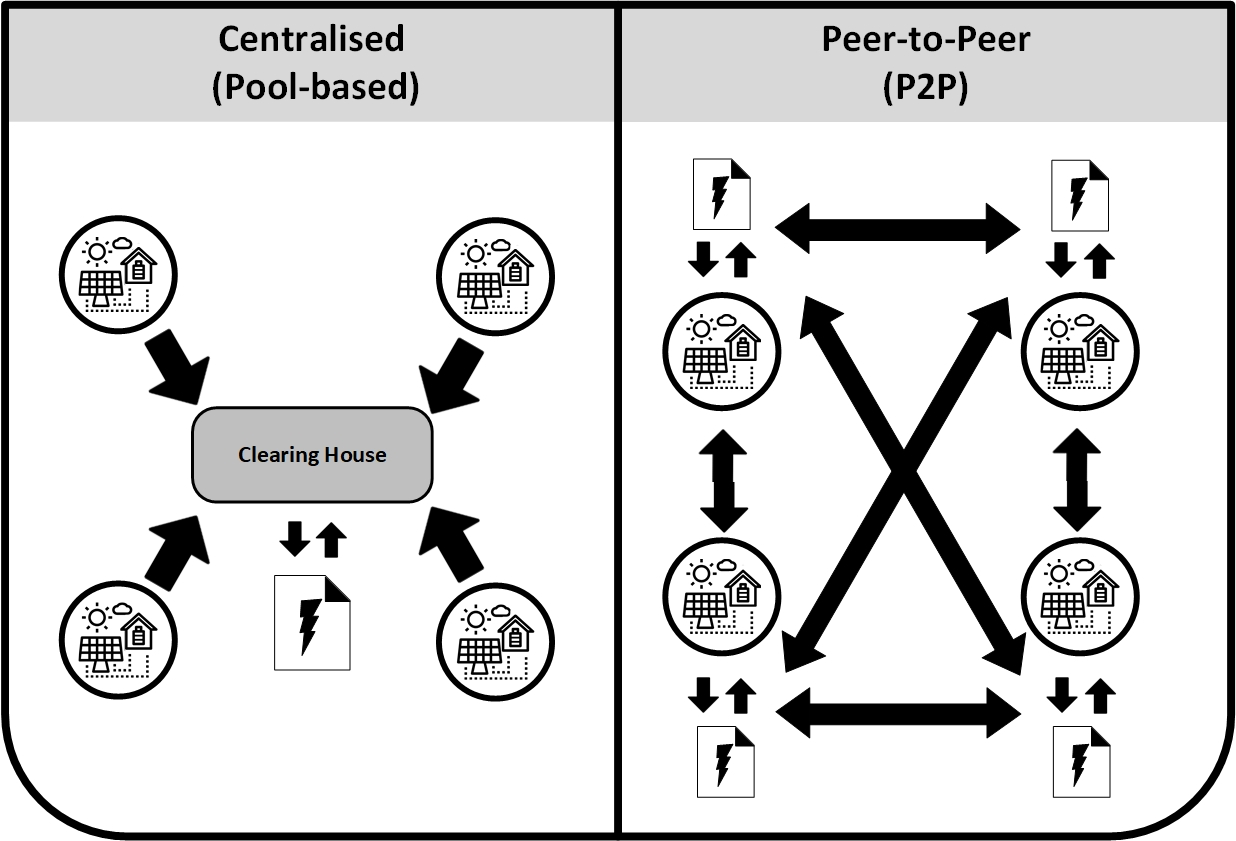
\includegraphics[width=0.7\columnwidth ]{ChapterIntro/Figures/CENTRALISED_P2P.jpg}
	   %\vspace*{-8cm}
		\caption{Centralized vs P2P market approach}
	\label{fig:POOL_P2P}  
\end{figure}

LEMs between prosumers and the DSO can also be developed based on a centralized approach \cite{faqiry2017distributed}. Here, a bilevel iterative auction is proposed and the DSO is the main stakeholder of the market, with aggregators as intermediate agents competing for energy. Nguyen et al. \cite{nguyen2010pool} proposed a new poolbased market platform for flexibility services. The LFM operator is called the DR exchange operator (DRXO), who collects offers and bids and is responsible for the market clearing procedure. In \cite{paschalidis2012demand}, a market-based mechanism was developed based on a centralized approach. The platform operator is the smart microgrid operator (SMO), and it offers regulation service reserves covering the commands issued by the wholesale market independent system operator, which is responsible for energy provision and reserves purchasing. The main participants in an LM operating under a centralized approach are the aggregators, central platforms, the DSO and the group of consumers-producers-prosumers, that is, the LEC members. The LEC members in the LM are recruited from the neighbourhood and organized by the central entity or platform. In that sense, it is important to state that participation in this initiative is purely voluntary. Once the LMs have been broadly implemented in different neighbourhoods, members of the same neighbourhood are able to
choose a different central entity.

Related to the LM participants who are located within the LEC, all members with DERs and flexible loads need to have local control functionalities that can be included in either the smart meter or a local controller to receive command signals from the central entity. This entity also includes communication tools to receive and send control signals and messages between LEC members and the SESP platform, and also to interact with the wholesale market, as will be further detailed in Section \ref{sec:interaction}.

To guarantee a proper development and operation of the LM, each LEC member who participates in the LM is responsible for fulfilling the contract that has been established previously. In that sense, direct negotiations between traders are not allowed. This central entity has a set of roles that should be taken into account to understand the centralized approach. It works as a local market operator, by organizing energy exchange, scheduling local resources, and operating the trading platform. The local market represents the community members when it interacts with the wholesale market. Also, it ensures that all the energy that has been purchased on the wholesale market is consumed by community members and all energy sold must be produced by the LEC. Furthermore, this balance must be constant during all periods, otherwise the central entity will pay deviation penalties. The SESP is responsible for collecting all contracts and offering to their members a brokering, clearing, and price settlement service. The presence of a supervisory node or agent simplifies market regulation and the interface between the local or micro market and the system operator and wholesale market \cite{moret2018energy}.

\subsubsection{Peer-to-peer}
The idea of direct interaction and direct trading between agents in power systems was discussed 20 years ago, in \cite{wu1999coordinated}, where the concept of multilateral bilateral trading was first stated. This is what is now known as peer-to-peer (P2P) electricity trading.

In the P2P approach, prosumers and consumers trade between each other individually and in a randomized order on a pay-as-bid basis \cite{mengelkamp2018blockchain}. In this case, different prices for each trade are possible, since P2P trade involves one-to-one transactions. The P2P approach in energy markets is based on blockchain technology. Blockchain originated in 2008 with Satoshi Nakamoto. Related to blockchain, bitcoin was created in 2009, becoming the first decentralized currency, now known as cryptocurrency. Blockchain can be defined as a distributed and digital transaction technology that allows secure storage of data and execution of smart contracts in P2P networks \cite{swan2015blockchain}. It is a distributed ledger system that instead of having a central entity responsible for coordinating, settling, and archiving, decentralizes this task and relies on a number of entities that work in parallel with a specific ledger copy \cite{Pinson2017}.
In addition, blockchain contains a continuously growing list of data records, which are called blocks. These blocks are time-stamped, shared, unalterable, and connected to preceding blocks. Blockchain blocks can contain data, programs, batches of individual transactions, and executables.

In terms of P2P energy markets, \cite{blouin2001decentralized} proposed a new decentralized market in which there is no auctioneer and transactions take place via pairwise meetings of agents. It could be understood as the first definition of a P2P approach in energy markets. P2P markets rely on a consumer-centric bottom-up approach by giving prosumers the opportunity to choose the energy source they want, based on expressed preferences \cite{sousa2018peer}. The first application of blockchain in electricity markets was developed in 2014 by \cite{mihaylov2014nrgcoin}. These authors proposed a new virtual currency (NRGcoin) for renewable energy trading, which is produced locally. NRGcoins are quite similar to bitcoins. The mechanism converts locally produced renewable energy directly to NRGcoins, independent of their value on the market. Consumption is measured and billed in near real-time, achieving a model that is closed to the current operation of the grid.

Regarding this market approach, few implementations have been developed in the field of energy markets. In \cite{al2015bitcoin}, a new decentralized market for carbon emissions trading based on bitcoin is detailed. Sikorski et al. \cite{sikorski2017blockchain} developed a proof-of-concept to enhance the machine-to-machine electricity market in the chemical industry, also based on blockchain. Related to this market approach, a pilot site based on blockchain as the main ICT was developed in the Brooklyn Microgrid Project \cite{mengelkamp2018designing}. A new architecture for microgrids is presented in \cite{munsing2017blockchains}, where the blockchain P2P approach is applied instead of a microgrid aggregator to manage the DERs within the microgrid. In \cite{mengelkamp2018blockchain}, a double-sided market based on the P2P blockchain approach is detailed. It does not use bitcoin protocol but instead applies the Ethereum protocol. Mannaro et al. \cite{mannaro2017crypto} analysed a blockchainbased software platform for P2P energy trading to enhance renewable energy integration and trading within the Sardinia region. Recently, a project called Enerchain \cite{Enerchain} has been set up to work on P2P energy trading in the wholesale market using blockchain technology. Using this approach for energy trading, the wholesale market operator is no longer needed. This project is comprises energy trading firms that take part in the wholesale market at the present time. The evolution of the power system leads to new market design, business models, and market approaches, and the path leads towards a fully decentralized power system, with different scenarios still opened. To that extent, and based on P2P electricity trading, in theory the power system could be based on consumers being able to choose directly the type of electricity source they want to buy and LECs that provide flexibility services to the system operator or to be traded within the same community. On the other hand, a power system based on LECs could provide a community feeling among the agents involved and trade on energy and flexibility as their main purpose or the energy could also be exchanged with external agents (other microgrids or consumers not located inside the LEC) or with the system operator, for example the DSO. There is a need to define the rules of each smart grid agent to avoid any conflict with the existing top-down power system structure, wholesale market, and additional electricity markets.


\subsection{Services} \label{sec:services}
The main aim of local electricity markets is to facilitate the transition towards a smart energy grid by connecting new or redefined smart grid agents thanks to new services provision. In this chapter, the literature review has introduced two different services that can be provided by a local market: energy trading and flexibility services exchange. These services can be provided separately or together between local market agents 

\subsubsection{Energy}
Most of the literature references we have found defined LEM for energy trading. According to \cite{ilieva2016design}, the objective of the energy service is to schedule local resources at minimum cost during the day ahead, achieving an equilibrium point between local demand, local supply, and grid exchange. First, an energy service is a way to sell and/or buy energy for customer purposes. The main concept to take from the local market for energy services is trading energy locally (from local resources inside the LEC) to reduce electricity consumption from the main grid.

Two LEM approaches are detailed in \cite{mengelkamp2018blockchain}: the P2P market and the closed order book market, with the aim of trading electricity directly within their community and concluding that the P2P LEM approach is the most advantageous, with the lowest energy prices. Later, in \cite{mengelkamp2017role}, a LEM case study based on P2P trading and bitcoin, without the need of central intermediaries, was developed. In this work a framework is also described, with seven market components for its efficient performance. Energy trading within a microgrid based on a P2P approach was developed in \cite{luo2014autonomous} to minimize the microgrid operation cost by increasing the integration of renewable DERs. In \cite{menniti2014future}, a new market platform was created to coordinate energy exchanges between micro-smart grids aggregated in a virtual energy district (VED). It is based on a centralized approach and the local market operator, the CEP, handles the supply and demand of prosumers within the VED. In \cite{Menniti2015}, the integration of distributed energy storage within the VED is analysed to improve the performance of the LEM.
Cui et al. \cite{cui2014electricity} considered a microgrid as a closed economy group and detail two market-based approaches. The first model deals with the optimal power generation per hour within the microgrid. The second model allows energy trading between microgrids for local welfare maximization.

Interactions and power exchanges between microgrids can also be considered as microgrid energy markets or micro markets. In \cite{Lee2015, Gregoratti2015}, market-based mechanisms are studied to schedule and exchange power flows between microgrids, to minimize the global operation cost. In \cite{ferruzzi2016optimal}, a prosumer acts as an aggregator within the microgrid and buys or sells the energy in the DAM. This paper considers the uncertainty provided by the DERs located within the microgrid. Cintuglu et al. \cite{cintuglu2015real} implemented a multiagent-based game theory auction market model that combines conventional and renewable DERs to schedule the microgrid resources. Staudt et al. \cite{staudt2017analysis} defined an LEM as a market set up to solve redispatch locally by providing economic incentives for the expansion of local capacity generation.
Prosumer clustering is a topic that is currently being addressed in the literature \cite{doulamis2017virtual, vergados2016prosumer, da2013impact}. This approach can enhance prosumer participation in local and micro energy markets. Prosumer clustering is an aggregation of prosumers through ICT platforms.
At a higher level, coordination of micro and local markets can also be considered as a local market \cite{menniti2014future}.

This new market aims to coordinate the energy exchanges between local and micro power markets. In \cite{zachar2016microgrid}, microgrid interaction with the macrogrid or distribution network is defined in a market-based approach. 
Storage and community energy storage (CES) are key elements in local and micro energy markets to achieve the optimal operation of the energy market and DERs located within the LEC \cite{Olivella2016ENERGYCON, Bayram2014, mengelkamp2017role, Menniti2015, menniti2014management, mediwaththe2017competitive}. Storage can be understood as units that are controlled by the local market operator to maximize the social welfare of the LEC \cite{Olivella2016ENERGYCON}. Results in \cite{mengelkamp2017role} indicate that LECs with CES have greater local market efficiency. 

The scheme in Figure \ref{fig:marketinteraction} exemplifies how an LEM can work. The LEC is represented by the grouping of different prosumers. This LEC can trade locally by means of an LEM operated by a local market operator or the aggregator. The LEM schedules the local resources depending on their market time horizon, usually the day-ahead. Then, if there is a surplus or a lack of energy resources based on the LEC's resources, the LEM can interact with the day-ahead wholesale market or intraday market to trade the energy needs.


\begin{figure}[]
	\centering
	\includegraphics[width=1\columnwidth ]{ChapterIntro/Figures/Figure2.8.jpg}
	   %\vspace*{-8cm}
		\caption{Local energy market interaction}  
	\label{fig:marketinteraction}
\end{figure}


\subsubsection{Flexibility}
Flexibility can be understood as DR or DSM activities, the so-called demand-side participation. As DERs are installed along the distribution grid, there is a need for end-user flexibility to maximize DER integration and their profitability. In addition, high flexibility is required to deal with the uncertainty of renewable generation and variability on the demand-side. An electric flexibility service can be defined as a power adjustment sustained at a given moment for a given duration from a specific location within the network \cite{Lee2015}. Flexibility activities reflect the possibility of modifying generation and/or consumption patterns in reaction to an external signal (price or activation) to contribute to the power system stability cost-effectively \cite{VILLAR2018Flexibility}. DR is considered to be the tool that will be used to achieve energy efficiency and intermittent RES goals, and where customers will play a crucial role. Thus, according to the previous definition, there are three types of DR actions, according to Albadi and El-Saldani \cite{albadi2008summary}:

\begin{itemize}
\item Electricity reduction. End-users reduce their electricity usage during critical peak periods when prices are
high, but they do not change their consumption pattern. This leads to temporary comfort losses. 
\item Load shifting. Consumers shift their consumption activities from peak demand periods to off-peak periods to respond to high electricity prices. To exemplify this, end-users shift their household activities (dishwashers, washing machines, electric vehicle (EV) charging) to lower-priced periods. In this case, there is no or little reduction of comfort. 
\item On-site generation. Consumers who generate their power by using DERs can follow their consumption profile without changing their behaviour, but by just swapping the origin of the electricity generation. In this case, they experience no or little change in their load profile but, from the utility point of view, a reduction of energy consumption will be noticed.
\end{itemize}

To sum up the characteristics of DSM and DR, Figure \ref{fig:2.9} collects the different tools under the ideas of DSM and DR. Here, DR is considered to be a type of DSM where a temporary reduction or increase in energy consumption is performed by the end-user. Energy efficiency is also grouped under DSM. In this case, energy efficiency covers all the measures or investments performed to achieve lower energy consumption.

\begin{figure}[]
	\centering
	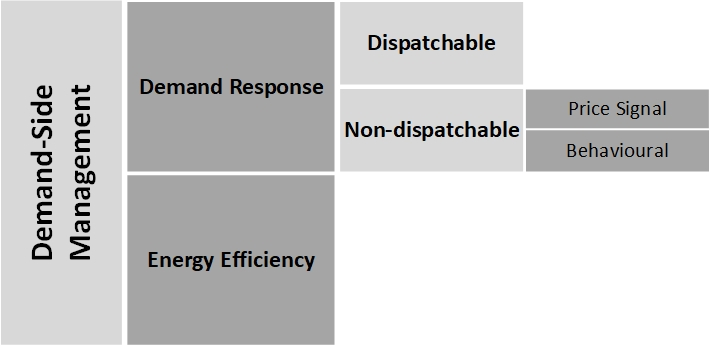
\includegraphics[width=0.8\columnwidth ]{ChapterIntro/Figures/DRDSM_BW.jpg}
	   %\vspace*{-8cm}
		\caption{Demand-Response and Demand-Side Management activities classification} 
	\label{fig:2.9}
\end{figure}

There are two types of DR: dispatchable and non-dispatchable. According to \cite{DNVGLEnergy2014}, dispatchable DR (DDR) refers to \textit{"planned changes in consumption that the customer agrees to make in response to a requirement from someone other than the customer. It includes direct load control of customer appliances and a variety of wholesale programs offered by RTOs/ISOs that compensate participants who reduce demand when directed for either reliability or economic reasons"}. For that reason, DDR can be considered as the participant giving the control of the loads to the utility, who is in charge of its management depending on the needs. Hence, dispatchable DR can be understood as direct control classical incentive-based programs in the DR classification defined in \cite{albadi2008summary}.

In non-dispatchable DR, participants choose if they want to change their behaviour. The utility sends information to the participant and it is the end-user who decides whether or not they follow the signal. Here, the participant remains the master of his loads and consumption. Two programs are included under nondispatchable DR: price-signal and behavioural. Price-signal is structured in the same way as time of use in a price-based program, where electricity price rates per unit consumption are defined. Behavioural DR is the
most innovative type of DR. ICT tools permitted the creation of this type of DR. Usually, participants in this program receive their energy consumption tracking (behaviour) thanks to smart meters, monitoring, and ICT tools. By using these tools, the participant can predict their energy use, reduce cost and also provide flexibility service to the utility, thanks to energy consumption tracking.
DR has a key role to play in helping to increase electricity system flexibility \cite{Cooke2011}. As a result, it will improve the efficiency of the power system, but also the efficiency of the electricity market and the power system security. A higher penetration of flexibility by DR programs will also help the integration of DERs, as DR can help to cover DER intermittency, achieving the goal of carbon footprint reduction (see Figure \ref{fig:2.9}).

The participation of consumers in DR activities can set up a proper market design to integrate flexibility services and increase market competition \cite{MarketDesignENTSOE}. Local flexibility services for the DSO and ancillary services for the TSO at local level can be provided on account of DER integration \cite{Roques2017}.

As a result of DSM and, more specifically, DR activities, flexibility comes into play. Flexibility can be used to adjust the demand profiles during peak periods, to adjust them to peaks of renewable generation, and, related to that, to the available capacity in the distribution grid.

A new framework to create markets for flexibility services has been defined in \cite{Ulbig2015,USEFFoundation2015a}: 'Demand response through load shifting and the storage and management of locally generated energy provides new means to unlock flexibility in the energy system'. In order to provide services to the power system operators, for instance the TSO or DSO, flexible resources and DERs are considered a group, facilitating their operability for flexibility services providing. The aggregator is then a key agent to add value to flexibility. It is responsible for aggregating the prosumers' flexibility, creating a flexibility portfolio and offering it to different stakeholders by means of diverse markets. The aggregator can then also offer services as a supplier and assume BRP responsibilities \cite{MarketDesignENTSOE}. Eurelectric states in \cite{mandatova2014flexibility} that there is a need for a new agent in the system, the flexibility operator and flexibility platform, which aggregates and coordinates the activation of flexible loads located along the distribution network. This market platform should facilitate coordination between the TSO and DSO, and minimize the cost of flexibility market participation. However, the impact of flexibility load participation in the market has to be analysed because it can lead to congestion in the distribution grid \cite{esterl2016impact}. The role of aggregators in DR programs is relevant in involving end-users in smart grid transition and providing ancillary services to system operators, both the TSO and the DSO \cite{Carreiro2017}.

Also in \cite{USEFFoundation2015a}, four potential customers are identified (Figure \ref{figure210}): the prosumer, the BRP, the DSO, and the TSO, managed by the aggregator as a central entity. Up to now, local markets for flexibility services have been mainly based on a centralized approach (Table \ref{tab:23}).

\begin{figure}[h]
	\centering
	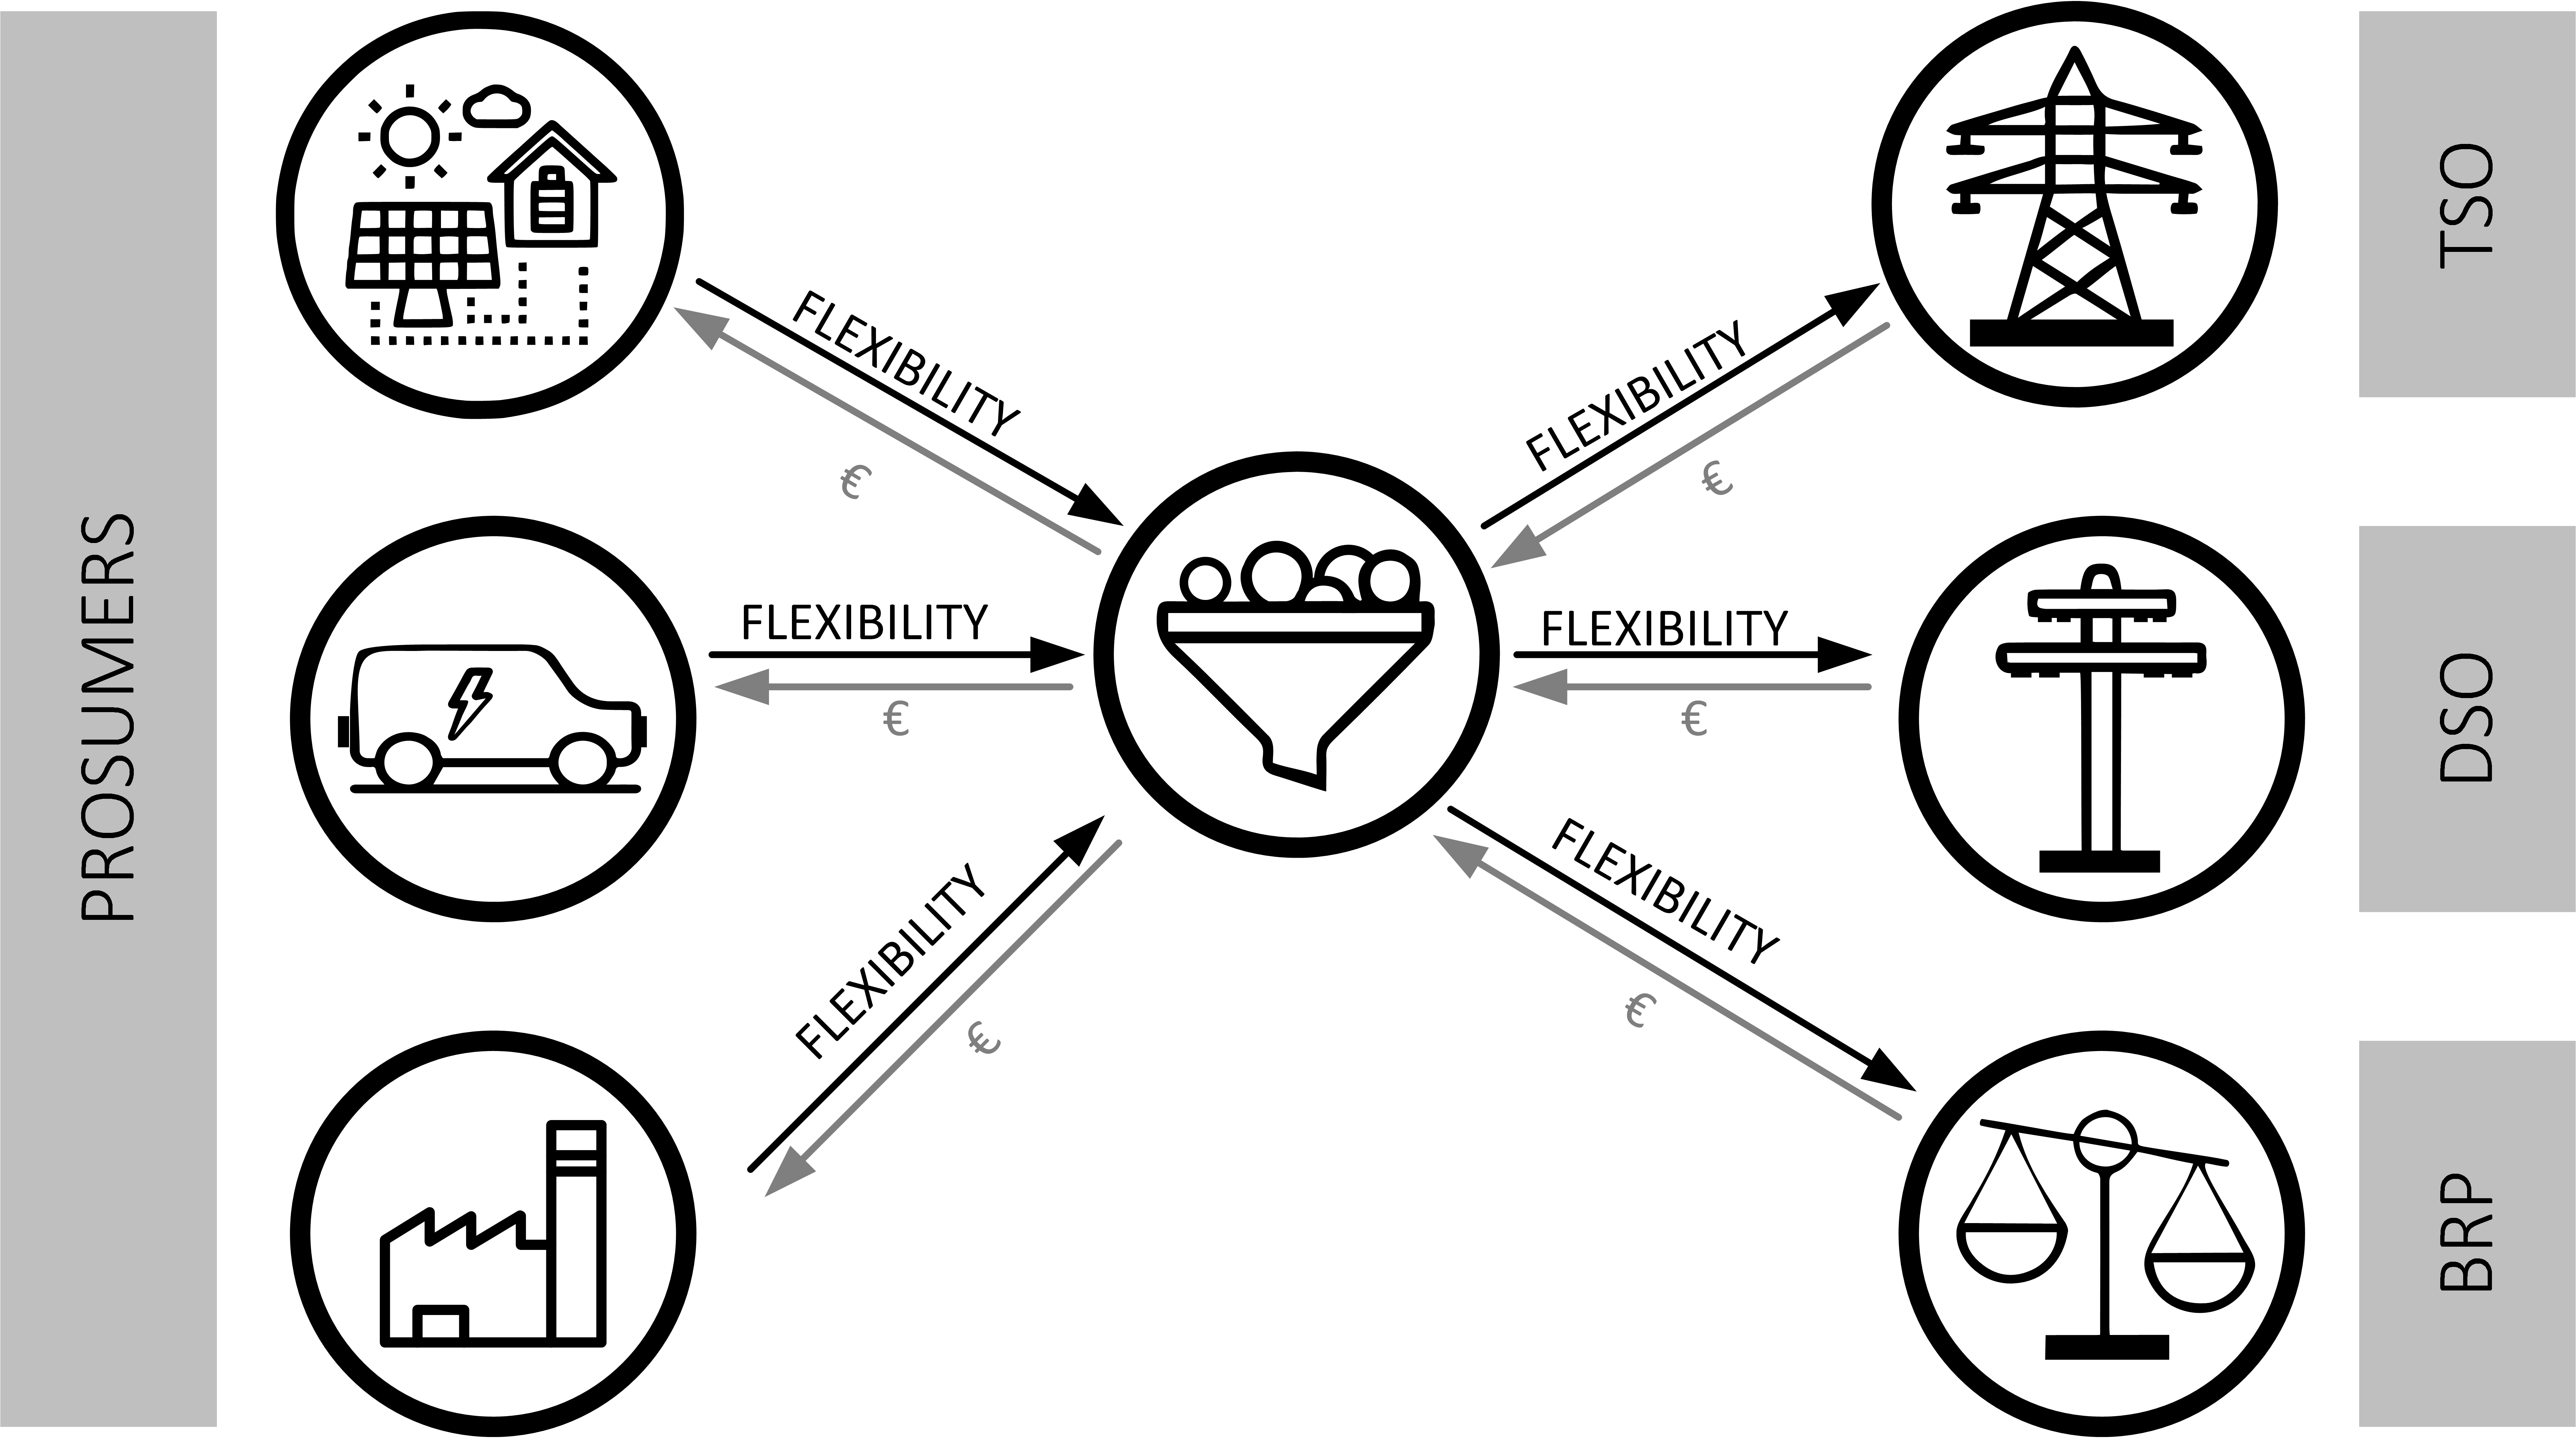
\includegraphics[width=0.9\columnwidth ]{ChapterIntro/Figures/Figure2.10.jpg}
	   %\vspace*{-8cm}
		\caption{Flexibility services and main stakeholders. Figure based on \cite{USEFFoundation2015a} }  
	\label{figure210}
\end{figure}

The market models proposed in \cite{USEFFoundation2015a, MarketDesignENTSOE} do not have an effect on the energy supply chain. They respect the European liberalized energy market model, but change the roles of the involved agents (Section \ref{sec:agents}) for these new services to be provided. The aggregator establishes a smart contract with the prosumer, optimizing the flexibility value in its portfolio and selling this flexibility to the stakeholder with the highest need for this service who is also willing to pay the highest price for it. It should be taken into account that here the role of the aggregator can be developed by a supplier or by an independent aggregator. In any case, they can take BRP responsibility or not.

Recently, several associations, such as Eurelectric, Groupement Europ\'{e}en des entreprises et Organismes de Distribution d'Energie (GEODE), the European Distribution System Operators Association for Smart Grids (EDSO for Smart Grids), and the European Federation of Local Energy Companies (CEDEC), have produced a report focused on the development of flexibility services for the DSO \cite{edso2018flexibility}. This report highlights the need for an improved regulatory framework that rewards the use of flexibility and also takes into account the evolving role of the DSO as an active system operator and neutral market facilitator. DSOs should be able to decide on the best solution to face challenges, either by activating flexibility services or by network reinforcement.

Figure \ref{fig:211} shows the entire supply chain with flexibility services integrated. At the top of the figure, the top line represents the energy flow from the generation plant to the transmission network, the distribution network and arriving at the consumers. Prosumers can also inject their small-scale generated power into the distribution network if regulation allows them to do that. As can be seen in the figure, the energy supply chain remains unalterable with the integration of flexibility services.

\begin{figure}[h]
	\centering
	\includegraphics[width=0.9\columnwidth ]{ChapterIntro/Figures/Figure2.11.jpg}
	   %\vspace*{-8cm}
		\caption{Flexibility services in a local flexibility market. Scheme and interaction}  
	\label{fig:211}
\end{figure}

The ticker line in the middle represents the flexibility flow. The aggregator settles a smart contract with the prosumer. This contract states the terms and conditions of the contracted flexibility services. Hence, the aggregator collects all the smart contracts, optimizes the flexibility assets portfolio, and then offers this flexibility to different stakeholders: the DSO, the BRP, and the TSO by means of the BRP. 

Lastly, the line at the bottom of the figure represents the economic flow between the different agents of the smart grid that combine energy and flexibility flows. The economical flow takes into account that the energy is sold and bought on electricity markets. The BRP is the entity responsible for the imbalances that are paid after the actual delivery. As a result, retailers, by means of the energy bill, are paid for the energy delivery to end-users. Furthermore, the BRP applies the imbalance payment to the final bill that the end-user is disbursing.

Current literature proposes different services offered by LFMs or local markets for flexibility services. Olivella-Rosell et al. \cite{Olivella2018} developed an LFM. In this the local market operator controls the LEC flexible resources (thermal loads, EVs, storage, etc.) during specific time periods and rewards the participants accordingly on their smart contracts. On the contrary, LFM can be understood as a trading platform to adjust the energy resources to correct forecasting errors or to increase the participant's profits in balancing markets \cite{ilieva2016design}. In \cite{diekerhof2017hierarchical}, an aggregator collects and optimizes the day-ahead and intraday scheduling of electro-thermal heating units within a city district to provide flexibility services to the DSO and BRPs. Ramos et al. \cite{ramos2016realizing} described three different local market designs for local flexibility services for DSO: participating in the existing wholesale market, creating an LFM, and contracting flexibility as a system reserve. Bilateral contracts for flexibility services based on thermal loads from residential DR are defined in \cite{boscan2016flexibility}. The optimization model is also detailed and presented in \cite{boscan2016flexibility}, taking into account consumer preferences so that end-users can select their own contract based on them. Specific topics directly related to flexibility services are currently addressed in the literature, such as aggregating flexible loads \cite{nayyar2013aggregate, pandvzic2013offering} and thermostatic loads \cite{alahaivala2017control}.

In \cite{leclercq2019network}, flexibility market-based schemes are defined for TSO-DSO coordination. Two LEMs are detailed: a local AS real-time market and a common TSO-DSO AS market model. The local AS real-time market considers balancing and congestion management services for the DSO and the TSO. The DSO operates the local market to solve distribution grid problems and then aggregates the remaining flexibility offers to the TSO markets. 

The TSO-DSO AS market model is also based on real-time dispatching. It is based in a local market operated by the DSO, but satisfies the needs for both the TSO and the DSO. The LFM can be established to provide flexibility services to the TSO. Teotia and Bhakar \cite{teotia2016local} defined the local electricity market concept as an ancillary services provider for the DSO and TSO by creating a new local market operator, an aggregator, and a local grid controller (LGC). The LGC is responsible for the management of the local grid resources, such as energy storage, combined heat and power, residential flexible loads, and DERs. In \cite{rosen2013auction}, an auction-based LEM for TSO ancillary services trading is detailed based on BRP enhancement. Also related to ancillary services, \cite{martinez2013active} developed a secondary market for ancillary services offered by active demand participation (prosumers) to minimize grid operation costs. Regarding ancillary services, \cite{menniti2014future} considers them as a possible service that the LEM could provide to the TSO and DSO.

Different projects and market designs for electric flexibility trading are reviewed in \cite{eid2016market}. First, the Power Matching City project developed a local market operator, Powermatcher, which is in charge of controlling the operation of household appliances located in the Netherlands by means of direct and semi-direct control. 
The flexibility services are offered by prosumers to the DSO and retailers. The Energy Frontrunners project developed a flexibility aggregator that acts as an intermediary between the flexible loads, the BRP, and the DSO. In this project, the aim of the flexibility trading is to reduce the PV panels' peak and so the peak load in the distribution network during the evening period. In Germany a local integrated utility is at the same time the retailer, the owner of the distribution network, and also acts as a flexibility operator. It is responsible for trading flexibility between the TSO and the utility that controls the flexible loads. Here there is no participation of the DSO, the retailer, and the prosumers; the local integrated utility controls the operation of these flexible
loads and also of the grid.

A P2P approach can also be used in LFM, but it is not widely applied. Chen et al. \cite{chen2017integrated} proposed a new market mechanism for EV parking lots to participate in real-time markets, based on smart contracts and a P2P approach. These flexible loads can adjust their demand and consumption behaviour according to DSO requirements and incentives. The Your Energy Moment project \cite{eid2016market}, also developed in the Netherlands, is based on dynamic pricing signals that consumers receive thanks to in-home applications. Both the DSO and the retailer are able to submit their price to the participant.

\section{Local Market Services and Approach Review} \label{sec:servicesreview}
As a summary of the literature review detailed before, Table \ref{tab:24} shows the published papers in terms of the services provided, the main stakeholder, and the market approach. This table aims to show an overview of the current status of local and micro power market technology.
%\setlength{\tabcolsep}{10pt} % Default value: 6pt
%\renewcommand{\arraystretch}{1.5} % Default value: 1
%\begin{table}[]
%\centering
%\caption{Local market services and approaches literature review}
%\label{table24}
%\resizebox{\textwidth}{!}{%
%\begin{tabular}{@{}lll@{}}
%\toprule
%\textbf{Service / Approach}           & \textbf{Peer-to-peer} & \textbf{Centralized} \\ \midrule
%\textbf{Energy}                       &  \cite{mengelkamp2018designing, sousa2018peer, lamparter2010agent, vytelingum2010trading, moret2018energy, Heidari2018, Bayram2014, Pinson2017, mihaylov2014nrgcoin, munsing2017blockchains,mannaro2017crypto, Enerchain, mengelkamp2017trading, long2017feasibility, pouttu2017p2p, sorin2018consensus, baroche2018exogenous}  &                    \cite{sousa2018peer, karnouskos2011demand, rosen2013auction, ampatzis2014local, menniti2014local, EuropeanNetworkofTransmissionSystemOperatorsforElectricityENTSO-E2015, ilieva2016design, staudt2017analysis, moret2018energy, menniti2014future, cui2014electricity,     shamsi2015economic, Bayram2014,Pinson2017, faqiry2017distributed, Menniti2015, Lee2015,Gregoratti2015, ferruzzi2016optimal, mediwaththe2017competitive, mengelkamp2017trading, holtschulte2017local, wu2015optimal, mohan2015online, mohan2016sortino, gui2017distributed,lezama2018local}   \\
%\textbf{Flexibility to TSOs}          &  -                     & \cite{nguyen2010pool, nordentoft2013development, rosen2013auction, ramos2016realizing, leclercq2019network, staudt2017analysis, USEFFoundation2015a, martinez2013active, eid2016market, olek2014local}                      \\
%\textbf{Flexibility to DSOs}          & \cite{eid2016market, chen2017integrated, kok2016society}  &                       \cite{poudineh2014distributed, zhang2014flech, gawron2014integra, zhang2013flex,  spiliotis2016demand, eid2016market, diekerhof2017hierarchical, mandatova2014flexibility, USEFFoundation2015a, Olivella2018, pavlovic2016sgam, leclercq2019network, ramos2016realizing, nordentoft2013development, nguyen2010pool} \\
%\textbf{Flexibility from Demand-Side} &   \cite{eid2016market, chen2017integrated, kok2016society} &                     \cite{validzic2017clean, pavlovic2016sgam, Olivella2018,  USEFFoundation2015a, mediwaththe2017competitive, eid2016market,  mohan2015online,  lezama2018local,  gawron2014integra, zhang2013flex, spiliotis2016demand, zhang2014flech} \\
%\textbf{Flexibility to BRPs}          &   \cite{eid2016market} &   \cite{validzic2017clean, nguyen2010pool, pavlovic2016sgam, Olivella2018, USEFFoundation2015a, diekerhof2017hierarchical, eid2016market, zhang2013flex}                       \\ \bottomrule
%\end{tabular}%
%}
%\end{table}

\begin{table}[htbp]
\centering
\caption{Local market services and approaches review}
\label{tab:24}
\resizebox{\textwidth}{!}{%
\begin{tabular}{@{}lll@{}}
\toprule
Service / Approach &
  Peer-to-peer &
  Centralized \\ \midrule
Energy &
  \begin{tabular}[c]{@{}l@{}}\cite{mengelkamp2018designing, sousa2018peer, lamparter2010agent, vytelingum2010trading, moret2018energy, Heidari2018, Bayram2014, Pinson2017, mihaylov2014nrgcoin}\\ \cite{munsing2017blockchains,mannaro2017crypto, Enerchain, mengelkamp2017trading, long2017feasibility, pouttu2017p2p, sorin2018consensus, baroche2018exogenous}\end{tabular} &
  \begin{tabular}[c]{@{}l@{}}\cite{sousa2018peer, karnouskos2011demand, rosen2013auction, ampatzis2014local, menniti2014local, EuropeanNetworkofTransmissionSystemOperatorsforElectricityENTSO-E2015, ilieva2016design, staudt2017analysis, moret2018energy, menniti2014future, cui2014electricity}\\ \cite{ shamsi2015economic, Bayram2014,Pinson2017, faqiry2017distributed, Menniti2015, Lee2015,Gregoratti2015, ferruzzi2016optimal, mediwaththe2017competitive, mengelkamp2017trading, holtschulte2017local, wu2015optimal, mohan2015online, mohan2016sortino, gui2017distributed,lezama2018local}\end{tabular} \\
Flexibility to TSOs &
  - &
  \cite{nguyen2010pool, nordentoft2013development, rosen2013auction, ramos2016realizing, leclercq2019network, staudt2017analysis, USEFFoundation2015a, martinez2013active, eid2016market, olek2014local} \\
Flexibility to DSOs &
  \cite{eid2016market, chen2017integrated, kok2016society} &
  \begin{tabular}[c]{@{}l@{}}\cite{poudineh2014distributed, zhang2014flech, gawron2014integra, zhang2013flex,  spiliotis2016demand, eid2016market, diekerhof2017hierarchical, mandatova2014flexibility, USEFFoundation2015a, Olivella2018}\\ \cite{pavlovic2016sgam, leclercq2019network, ramos2016realizing, nordentoft2013development, nguyen2010pool}\end{tabular} \\
Flexibility from Demand-Side &
  \cite{eid2016market, chen2017integrated, kok2016society} &
  \begin{tabular}[c]{@{}l@{}}\cite{validzic2017clean, pavlovic2016sgam, Olivella2018,  USEFFoundation2015a, mediwaththe2017competitive, eid2016market,  mohan2015online,  lezama2018local,  gawron2014integra}\\ \cite{zhang2013flex, spiliotis2016demand, zhang2014flech}\end{tabular} \\
Flexibility to BRPs &
  \cite{eid2016market} &
  \cite{validzic2017clean, nguyen2010pool, pavlovic2016sgam, Olivella2018, USEFFoundation2015a, diekerhof2017hierarchical, eid2016market, zhang2013flex} \\ \bottomrule
\end{tabular}%
}
\end{table}

As shown in Table \ref{tab:24}, research has been focused mainly on centralized platforms to deal with local and micro power markets. Furthermore, the main services provided have been energy. For instance, \cite{ilieva2016design} has shown as part of the H2020 project EMPOWER how an LEM can exist side by side with a centralized platform that enables power exchanges. Cui et al. presented a market model for microgrids (micro market) with two different approaches \cite{cui2014electricity}. First, the microgrid is considered as a standalone entity and the central entity schedules the generation for it. The second approach is based on interconnecting close microgrids to trade between them to increase the total welfare, thanks to covering the local demand with local generation. Shamsi et al. solved an economic dispatch (ED) problem for resources scheduling within a microgrid by means of a dynamic ED algorithm for each agent \cite{shamsi2015economic}. It is based on a centralized approach, since there is a microgrid market operator who is responsible for collecting microgrid agents' offers and bids and finding the microgrid spot price. A micro market within a microgrid, using a centralized approach (the microgrid service provider), is theoretically defined in \cite{gui2017distributed}. This central entity is one where community users can acquire the services. It emphasizes the democratic and community feeling on which the microgrid community is based.

In \cite{moret2018energy} an energy collective is presented based on both the P2P and centralized approaches. A community of prosumers is considered, and they are responsible for scheduling their resources using their own priority rules (no social welfare considered of the whole community), that is, behind-the-meter. They can trade the lack or excess of energy by means of a central entity called the community manager. The community manager is also able to directly interact (P2P) with other community managers to trade energy. The community manager is also the smart grid agent who interacts with the market and system operator, as well as being the supervisor of convergence to system optimality. Mengelkamp et al. \cite{mengelkamp2017trading} introduced and compared four scenarios for an LEM. They are based not only on two market approaches, P2P and centralized, but also considering zero intelligence agents and intelligently bidding agents. The research concluded that P2P markets considering intelligent market agents reach a lower average electricity price for the community.

Based on a P2P market approach, in 2014 Mihaylov presented a novel mechanism for energy trading: NRGCoins \cite{mihaylov2014nrgcoin}. They were formulated as a virtual currency for renewable energy injected into the grid, which was later traded between prosumers by means of blockchain technology. Sorin et al. \cite{sorin2018consensus} introduced multilateral energy trading taking into account product differentiation. In this case, the product differentiation covers consumer preferences. It allows prosumers participating in this market to be more involved and proactive due to the possibility of increasing their interest regarding energy origin and typology. One of the drawbacks that is highlighted in this paper and has to be taken into account when working on P2P electricity markets is the scalability of them. The computational costs for scaling a P2P market are higher than for a poolbased market. The latter is considered to be far more structured than P2P trading, thanks to the intermediary that negotiates with the agents involved in the LEC and also to external agents such as the system operator, aggregator, or BRP. A solution proposed in \cite{sorin2018consensus} to increase the scalability of P2P markets is to reduce the communication between agents participating in the market. In order not to rely on any central entity, a blockchain-based microgrid energy market is presented in \cite{munsing2017blockchains}, with the aim of guaranteeing that payments are made between non-trusting microgrid agents. By means of the alternating direction method of multipliers optimization method and local optimal power flow, a set of batteries, and curtailable and shiftable loads located along the distribution grid are scheduled. When dealing with LEMs based on a P2P approach, one of the most important shortcomings is where to allocate the grid costs. Baroche et al. \cite{baroche2018exogenous} present a method to
allocate grid cost based on the electrical distance between market participants. In this approach an ED along with product differentiation is carried out. In many literature papers the ED was done but without taking into account the grid infrastructure.

The fact is that P2P has an impact on the grid status, and the grid status and electrical distance should have an impact on peer interactions. Hence, in this paper, by applying electrical distance cost allocation there is a reduction in power trades between agents because the proposed market mechanism pushes the market agents to consider and respect the power system capacity constraints.
Several projects are currently ongoing in Europe in the field of local and micro energy markets, as stated in \cite{sousa2018peer}, mainly focused on the interaction between prosumers and consumers based on DERs located in a low voltage distribution grid. Local control and ICT platforms are a core part of these projects and both centralized \cite{ilieva2016design} and P2P \cite{moret2018energy, Enerchain, mihaylov2014nrgcoin} approaches are being used to implement the market design.

In terms of flexibility, it is worth separating them into the agents involved in the flexibility services chain. In this case, four distinctions are made: TSO, DSO, BRP, and prosumers. As can be seen from Table \ref{table24}, the centralized approach has also been the main research focus in the field of flexibility services. 

The main actor in receiving flexibility services is the DSO. Due to the increase in DERs and the need for grid capacity enhancement, the DSO needs market tools to facilitate their operation in terms of congestion management. Ramos et al. present three main approaches to contract flexibility: by means of the already existing wholesale market, by creating a new LFM based on a centralized approach, and a reserve market approach, contracting flexibility as a system reserve \cite{ramos2016realizing}. iPower is a project supported by the Danish Government with the aim of innovating and investigating intelligent power. The development of a DSO market for flexibility, by means of DR schemes and based on the aggregator role to collect end-user DR for DSO purposes, is introduced in \cite{nordentoft2013development}. The specifications in terms of flexibility services to be provided by end-users are detailed, such as the size of the service in power, the service in energy, the maximum duration of service per activation, pricing, and penalty. In 2017, another H2020 European project called INVADE began \cite{Olivella2018} with the aim of developing a centralized local flexibility trading platform to sell and buy flexibility within a specific area.

In this platform, the aggregator acts as a central entity and also as an esco. In this project, prosumer flexibility is aggregated by means of the flexibility operator or aggregator, and so it is responsible for participating in the market. This central entity aims to maximize the profits for its prosumer portfolio. Thanks to the flexibility provided by prosumers, the central entity can provide new services to the two main actors in the smart grid: the BRP and the DSO. The use of DR schemes for providing flexibility services to the DSO is analysed in \cite{spiliotis2016demand, poudineh2014distributed} based on a centralized approach.

Flexibility services provided by means of P2P trading are still not implemented as much as the centralized approach. However, Kok et al. \cite{kok2016society} describe a P2P mechanism based on transactive energy to provide flexibility services to the DSO to maintain the distribution network resiliently and efficiently. The mechanism was initially focused on the USA but the PowerMatcher project is ongoing to implement transactive energy trading by giving the consumer and prosumer the role of deciding whether or not to sell flexibility to parties involved in the project. Chen et al. describe a trading mechanism based on P2P to encourage users with flexible loads as EV to adjust their charging behaviour according to DSO requests \cite{chen2017integrated}.

Table \ref{table24} proposes a classification of existing literature in local and micro power markets, considering energy and flexibility as services to be provided and P2P and centralized as approaches to providing these services. This is a topic of current interest and much research is being carried out at present. The roadmap of this technology is evolving from a theoretical framework to even more research and implementation to prove its feasibility. There is still research to be done and questions to be answered, such as the viability of P2P mechanisms for providing flexibility.

\section{Local Market Interaction} \label{sec:interaction}
In this chapter different local market services and structures have been presented. The fact that local markets provide energy and flexibility exchanges may lead to interactions between these new local markets and existing energy markets worldwide. A possible general interaction among these markets is outlined in Figure \ref{fig:212}, based on a centralized approach by a central platform. To run these markets, local traders need this platform for sharing information, trading energy and flexibility, and scheduling actions. The smart energy platform acts as a local market facilitator for the LEC and also as an aggregator for wholesale market agents. The platform takes actions to increase market interactions, ensuring liquidity. Moreover, LMs could have problems balancing consumption and generation using only local resources, in terms of energy. Hence, it is imperative for the central platform to operate in wholesale markets during such periods to buy or sell the community energy deficit or surplus.

\begin{figure}[]
	\centering
	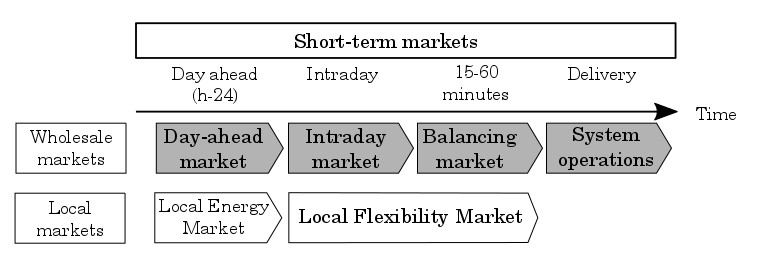
\includegraphics[width=0.9\columnwidth ]{ChapterIntro/Figures/LM_WSM_Interaction.jpg}
	   %\vspace*{-8cm}
		\caption{Wholesale and Local Market interaction in the short term. Based on \cite{InternationalEnergyAgency2016}}
	\label{fig:212}  
\end{figure}


The energy and flexibility LMs have their parallels in the wholesale market. The negotiation period of the LEM is equivalent to the DAM, and the LFM is equivalent to intraday plus the balancing market, as shown in Figure \ref{fig:212}. The reader should take into account that the scheme shown in Figure \ref{fig:212} is one possible option to define the interaction between local and micro power markets and existing wholesale markets. In this chapter we propose an interaction scheme, but there are several options to define the integration between markets. The following chapters examine the different structures. In Chapter 3, specific interactions between micro markets
and wholesale markets are presented and in Chapter 4 the interaction between local markets and wholesale
markets is covered.

As shown in Figure \ref{fig:212}, the first market that is being run or that starts is the LEM. With the aim of maximizing the community benefits for the LEM from the DAM, the central entity asks their members to participate in the LEM. It starts one day before the delivery or operation day, and the central entity estimates local energy consumption to determine if the LEC has to purchase or sell electricity in the DAM. The SESP prepares bids and offers for the DAM with the objective of minimizing energy costs. In addition, this central entity also is able to schedule flexible loads to reduce energy costs or, on the contrary, maximize LEC benefits.
Thus, the SESP prepares the corresponding bids, which include transactions between local consumers and producers within the same LEC.
Additionally, the energy bid must be within the distribution limits defined in the DSO-SESP contract. It should be taken into account that in European electricity markets bidding in the DAM is a prerequisite for wholesale market participants to get access to intraday and balancing markets such as OMIE or NordPool. The result of executing the LEM is that the energy plan that contains information about energy purchased or sold after the DAM auction during each period by the entire community. The following section outlines the steps needed to obtain the energy plan.

Once the energy plan is settled for the operation day, the trading platform shifts to the LFM. In the LFM, the central entity or aggregator controls its members' flexible resources such as loads, generators, EVs, and batteries during certain time intervals and rewards them according to their flexibility contract activation prices. Flexibility contracts for loads, EVs, and batteries are explained in detail in \cite{Olivella2018}. The LFM defines flexibility plans according to allocated and reserved flexibility for future needs. The goal of the LFM can be summarized as follows: it should comply with DSO requests to prevent grid overloads caused by consumption
or generation from community members or others connected to the same grid. Thus, the LFM allows the DSO to prevent grid damage and postpone grid reinforcements. It should compensate for BRP deviations due to forecasting errors or other issues to reduce deviation penalties for the BRP in wholesale markets. The aggregator uses the ICT platform to send flexibility control signals to compensate for LEC deviations if the deviation penalty is higher than the flexibility costs. Last but not least, the LFM should also comply with
prosumer needs. In the case of no external request, the aggregator can activate flexibility to reduce electricity cost individually.

All LFM participants need to have a contract with the aggregator. Nowadays, consumers can have separate or unified contracts with the BRP for consuming and producing electricity depending on the national regulations. Additionally, the LFM adds a new contract for activating flexibility. Local flexibility market participants settle an activation price for every flexibility asset, and they can include additional constraints like permitted activation periods or the number of flexibility activations per day. These contracts can be renewed every month, week or day depending on participation levels. The aggregator issues all contracts and offers a
brokering, clearing, and price settlement service. The LFM algorithm is an optimization problem that minimizes the cost involved in scheduling the required flexibility. It can be formulated as a single-side auction between flexibility providers and the SESP, who will request flexibility to maximize social welfare. On the other hand, the algorithm could be implemented as a minimization cost for the SESP allocating the cheapest flexibility offers. Hours before the operation day begins, the SESP executes the LFM algorithm.

\section{Conclusions and Discussion} \label{sec:conclusions}

The power system is evolving towards a decentralized system, becoming democratized and user-centred, thanks to new developments in RES. The deployment of microgrids and LECs facilitates the integration of DERs along the distribution networks and local and micro power markets enable their remunerated operation. Until now research has been focused on the theoretical analysis of the definition and operation of local and micro power markets, without a clear distinction of both concepts and their boundaries. This has led to several ongoing projects that implement and prove this technology. As a result of this, a standardized terminology should be developed because there are differences between local and micro power markets regarding the typology, services, and participants.
In this chapter two different concepts have been presented, local power markets and micro power markets, that provide two types of services: energy and flexibility. The agents involved and the main stakeholders of local and micro power markets are described. A literature review is included to analyse the current state of the art of this technology, analysing the contributions on each type and service provided.

Local and micro power markets is a topic that has been discussed for many years, starting as a research idea with many limitations and shortcomings \cite{wu1999coordinated, blouin2001decentralized, lund2006integrated, alibhai2004distributed}. However, there is an important shortcoming regarding regulation, since many countries do not allow energy to be traded locally, especially if it is based on P2P trading \cite{DesignElectricityMarketRossetoo2017}. 

Flexibility is a product that the current regulation is enhancing with the creation of the aggregator figure, allowing the grid active management as well as the end-user engagement at the same time. This is the product that will be considered for achieving the enery transition objectives presented in this research. The following chapter will go deeper into the definition of flexibility, which will be either traded in a bilateral contract or a centralized market. More detailed regulatory aspects of local and micro power markets will be developed in the following chapter. Apart from the technical benefits of local and micro markets, they also allow the creation of a large number of novel business models by providing different products and services within the LEC or microgrid. 
	


